\chapter{The COMPASS Experiment} 
\label{Chap::compass}
\ifpdf
\graphicspath{{Chapters/COMPASS/Figs/Raster/}{Chapters/COMPASS/Figs/PDF/}{Chapters/COMPASS/Figs/}}
\else \graphicspath{{Chapters/COMPASS/Figs/Vector/}{Chapters/COMPASS/Figs/}} \fi

The COmmon Muon Proton Apparatus for Structure and Spectroscopy (COMPASS)
experiment is a fixed target experiment at located on the French side at CERN.
COMPASS started taking data in 2002 in the same hall as earlier Euopean Muon
Collaboration (EMC), New Muon Collaboration (NMC) and Spin Muon Collaboration
(SMC) experiments.  COMPASS has studied hadron structure through (SI)DIS,
Drell-Yan and Primakoff reactions and has done hadron spectroscopy measurements.
\par

The COMPASS spectrometer is a two-stage spectrometer.  The two stages are in a
series and each stage contains various tracking detectors and as well at the end
of each stage there is a muon wall filter for distinguishing between muons and
other particles.  Both stages also contain an electromagnetic and hadron
calorimeter.  Each stage is centerend around a strong spectrometer magnet used
for determining particle momentum.  The first stage downstream of the target is
the large angle spectrometer (LAS) and it is centered around the SM1 magnet
which has an integrated field of 1~Tm.  This stage detects tracks with larger
polar scattering angles roughly between 26 mrad and 160 mrad.  The second stage
is the small angle spectrometer (SAS) and it detects particle tracks having a
scattering angle between roughly 8 mrad and 45 mrad.  This stage is centered
around the SM2 magnetic which has an integrated field of 4.4~Tm.  A graphic of
the 2015 setup is shown in Fig~\ref{fig::compassSpec}.\par

\begin{figure}[h!t]
  \centering
  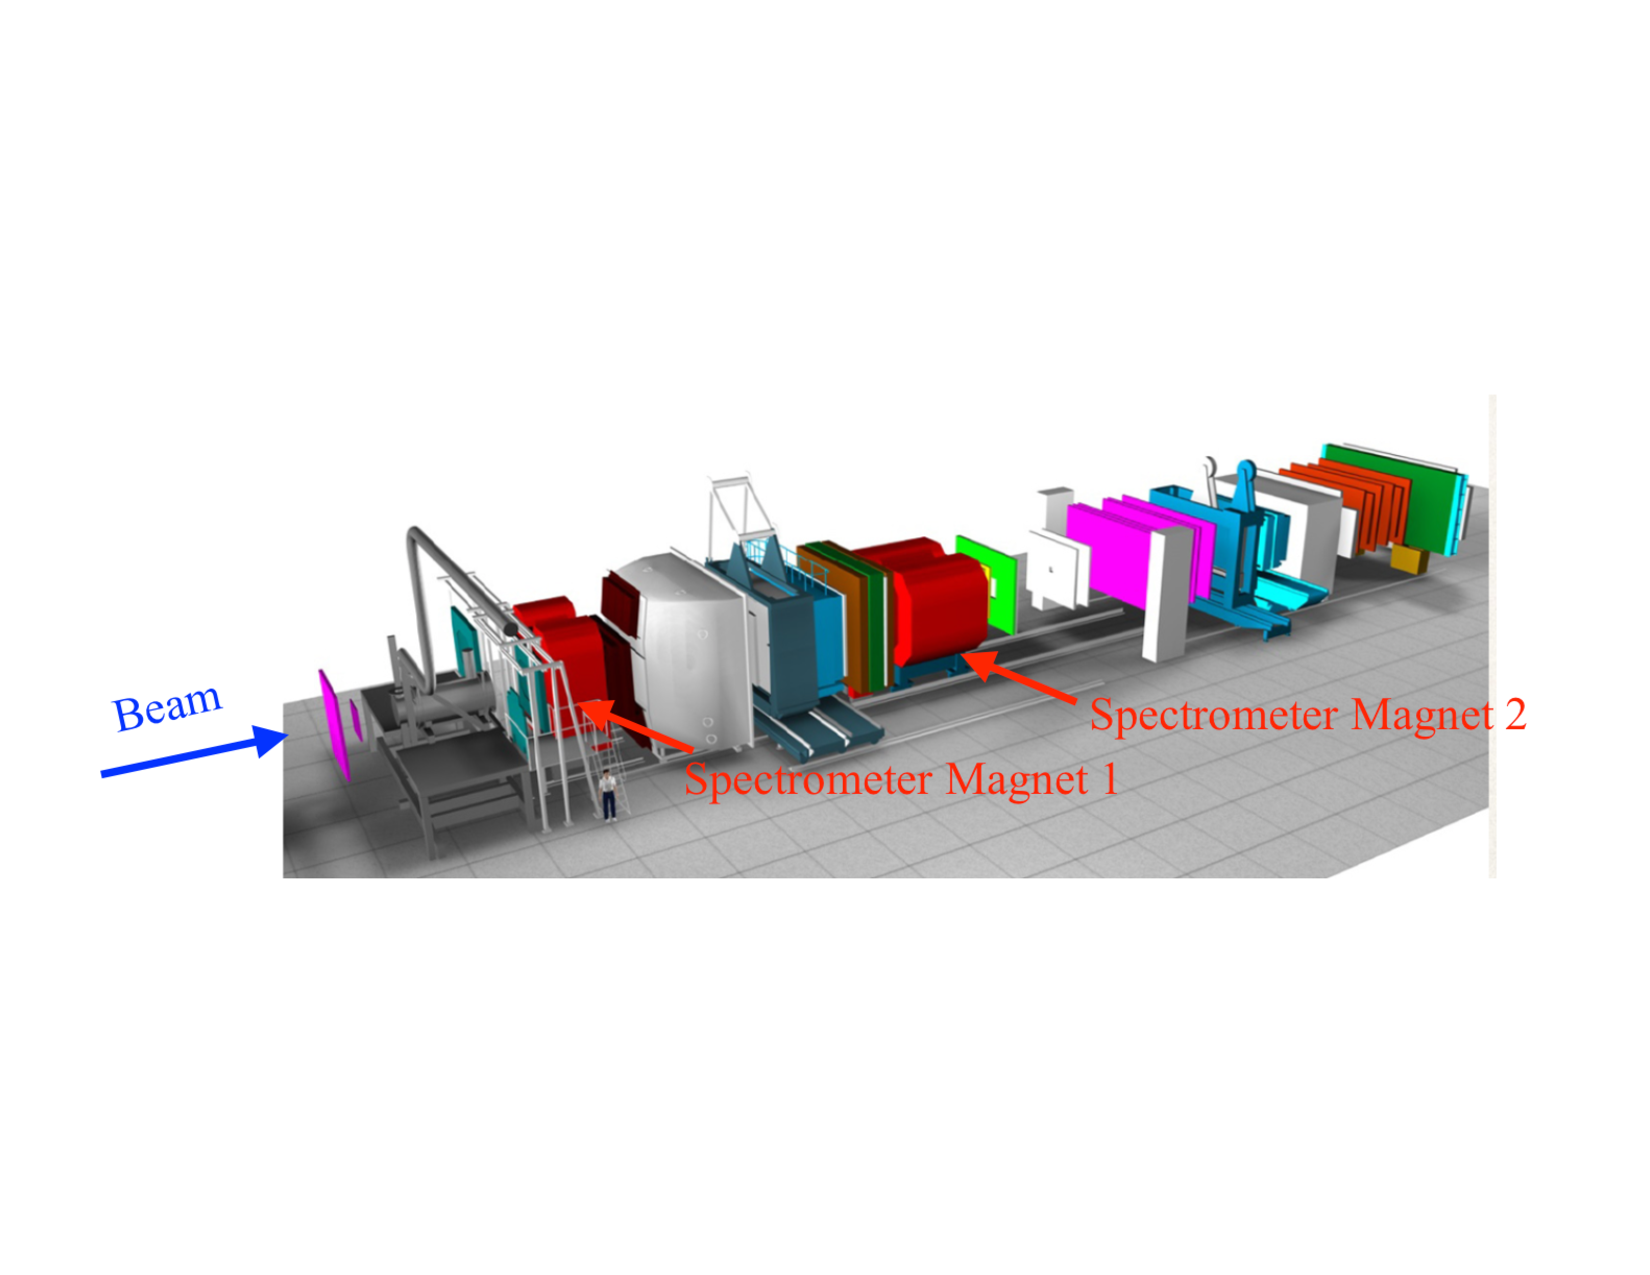
\includegraphics[width=\textwidth, trim=0.5cm 5cm 0.7cm 7cm,clip]{compassSpec}
  \caption{A schematic of the 2015 COMPASS setup}
  \label{fig::compassSpec}
\end{figure}

This chapter gives an overview of the COMPASS data taking setup with specific
interest on the 2015 setup from which the data in this thesis was produced from.
For a more thorough review of the spectrometer see
reference~\cite{compassSpec}.  This chapter is roughly organized by how the
data taking occurs.

\section{The Beam}
The COMPASS spectrometer receives beam from the Super Proton Synchrotron (SPS)
along on the M2 beam line.  The Super Proton Synchrotron (SPS) is the second
largest accelerator at CERN with a circumference of almost 7 km and it can
accelerate protons up to an energy of 450~GeV.  The SPS extracts beam to the
Large Hadron Collier and as well sends beam to various experiments in the North
Area at CERN.  A schematic of the M2 beam line is shown in
Fig.~\ref{fig::M2line}.  There are several different beam types and energies
available to COMPASS.  The most common types used for physics analysis are a
tertiary muon beam up to 190~{\gvc} and secondary hadron beam with an energy up
to 280~{\gvc}.  Both of these beam types can have a positive or negative charge.
As well it is possible to have a lower intensity tertiary electron beam which is
manly used for calibrations. \par

\begin{figure}[h!t]
  \centering
  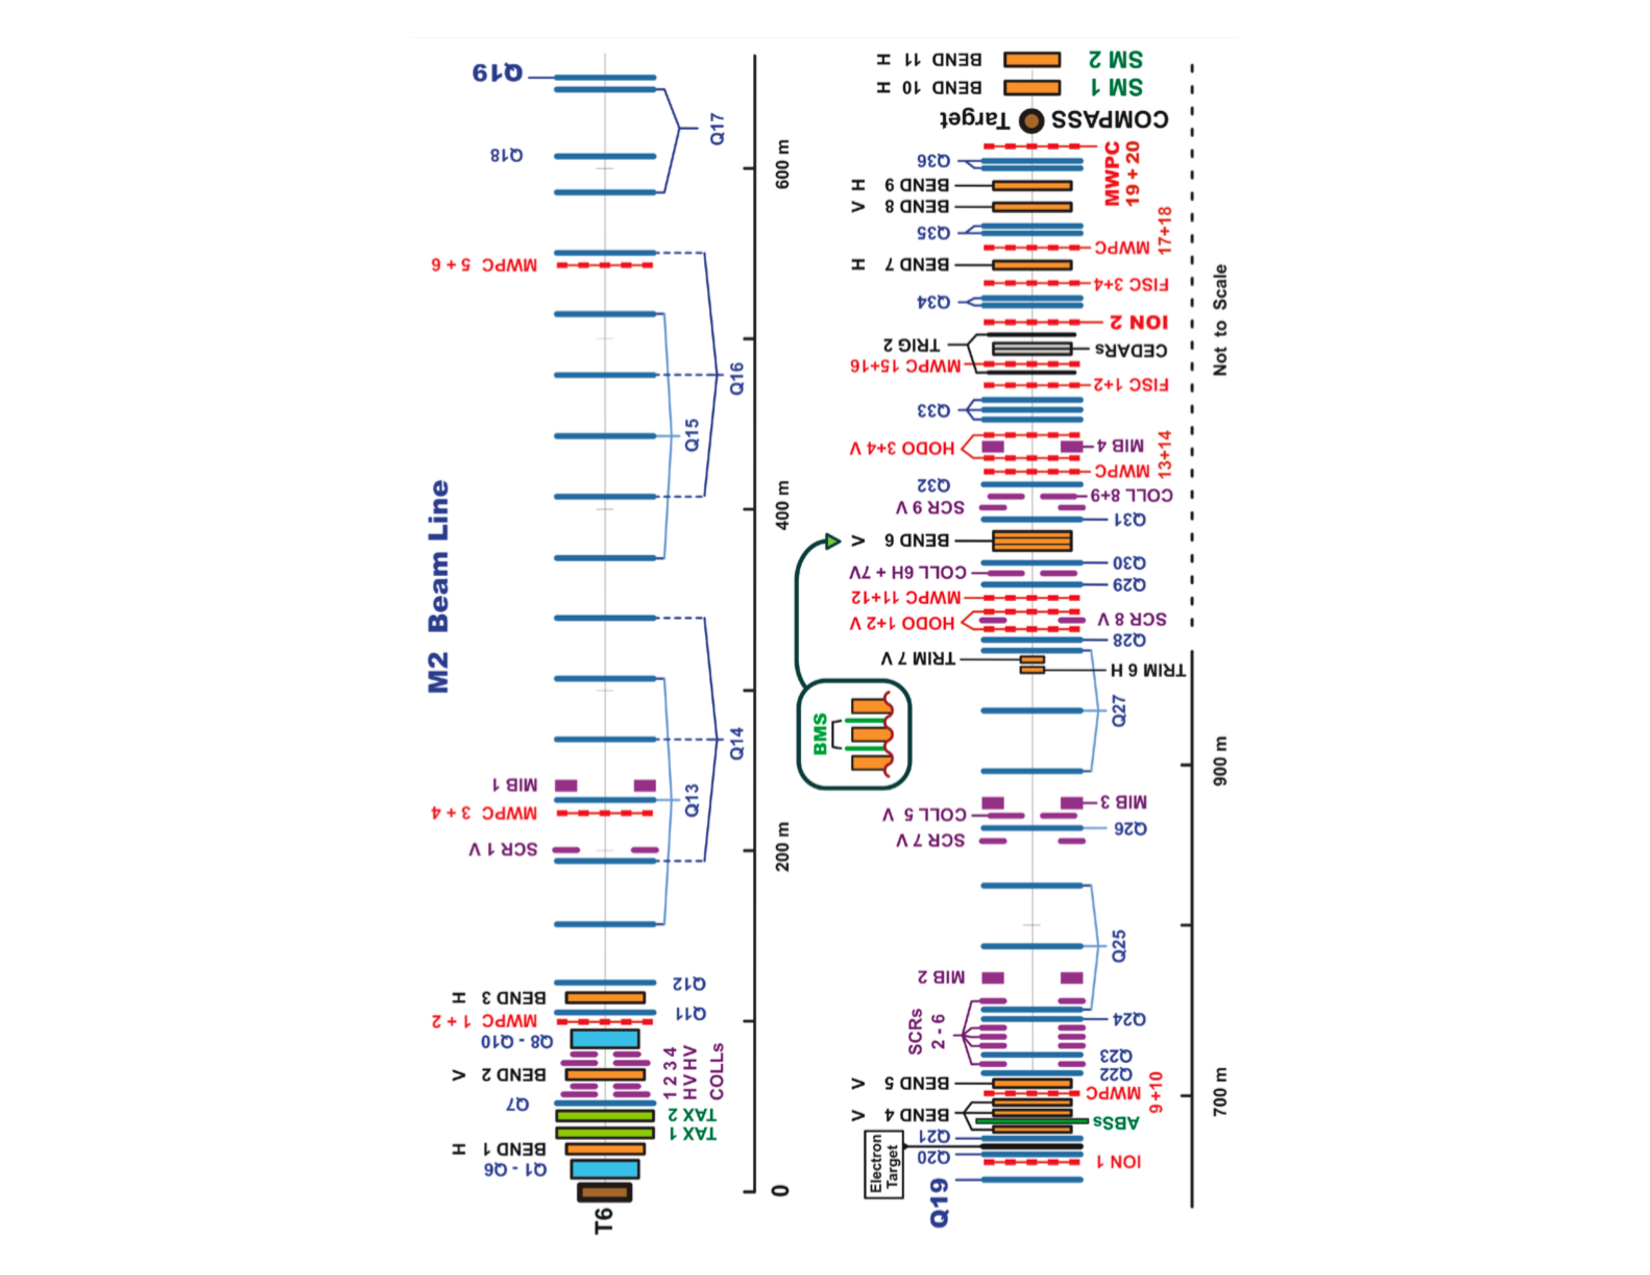
\includegraphics[width=\textwidth,trim=2cm 0cm 6cm 0cm,clip,angle=270]{M2line}
  \caption{The M2 beam line at CERN}
  \label{fig::M2line}
\end{figure}

The start of the M2 beam line is the T6 target which is made of beryllium and
has an adjustable length.  The SPS accelerates primary protons up to 400~{\gvc}
which impinges on the T6 target to produce a secondary beam.  The nominal proton
intensity on the T6 target is 100x10$^{11}$ spill$^-1$.  The longer the T6
target the higher the secondary intensity where 500mm is the longest and typical
target length used for physics data taking.  The reaction of the proton beam
with the T6 mainly produces secondary protons, pions and kaons.  Following this
reaction a series of dipole and quadruple magnets are used to select the
momentum and charge of interest. \par

The SPS spill structure varies throughout the data taking year depending mainly
on the needs of the Large Hadron Colider (LHC).  In 2015 the average intensity
provided was 0.6x10$^8$ s$^{-1}$ and the typical spill structure was two
4.8~second spills every 36~seconds.

\subsection{Muon Beam}
The muon beam is a tertiary beam which results from a weak decay of the
secondary beam.  After the initial proton reaction on T6 the resulting secondary
particles are momentum and charge selected and sent through a 600m tunnel with
focusing and de-focusing (FODO) quadruple magnets.  In this tunnel the pion and
kaons can decay as
\begin{equation}
  \pi^{-(+)} \rightarrow \mu^{-(+)} + \overline{\nu}_{\mu^-}(\nu_{\mu^+})
  \label{eqn::pionDecay}
\end{equation}
\noindent
and
\begin{equation}
  \kappa^{-(+)} \rightarrow \mu^{-(+)} + \overline{\nu}_{\mu^-}(\nu_{\mu^+}).
  \label{eqn::kaonDecay}
\end{equation}
\noindent
At the end of the tunnel a series of nine 1.1m long beryllium absorbers,
referred to as the ABS in Fig.~\ref{fig::M2line}, remove the remaining hadron
component of the beam which did not decay.  A 172~{\gvc} secondary beam is
chosen to achieve a 160~{\gvc} tertiary $\mu$ beam.  Due to the fact that the
neutrino in the reactions \ref{eqn::pionDecay} and \ref{eqn::kaonDecay} is
always left handed, the muon will be natural longitudinally polarized.  For the
muon momentum chosen the muon beam achieves a polarization of 80\%.

\subsection{Hadron Beam}
In the case of a hadron beam the ABS absorbers are not used and the decayed
muons are removed due to their lower momentum.  In the case of a negative hadron
beam the composition of the beam is approximately 97~\% $\pi^-$, 2.5\% kaons and
0.5\% $\overline{\mathrm{p}}$. The 2015 Drell-Yan data taking used a 190~{\gvc}
hadron beam. \par

\subsection{Additional Beam Line Components} \label{sec::addBeam}
After the decay tunnel the beam is bent upwards along another FODO tunnel of
length 250m before reaching the surface approximately 100m before the COMPASS
target.  A series of three dipole magnets, called bend 6, then bend the beam to
a horizontal position aimed at the COMPASS target.  Both upstream and downstream
of bend 6 are three tracking detectors (BM01-BM06) that make up the Beam
Momentum Station (BMS).  The BMS is the upstream most component of the COMPASS
spectrometer and is able to determine the beam momentum to better than 1\% of
the beam momentum with an efficiency of approximately 93\%.  Bend 6 and the BMS
are shown schematically in Fig.~\ref{fig::BeamLine1}. \par

\begin{figure}[h!t]
  \centering
  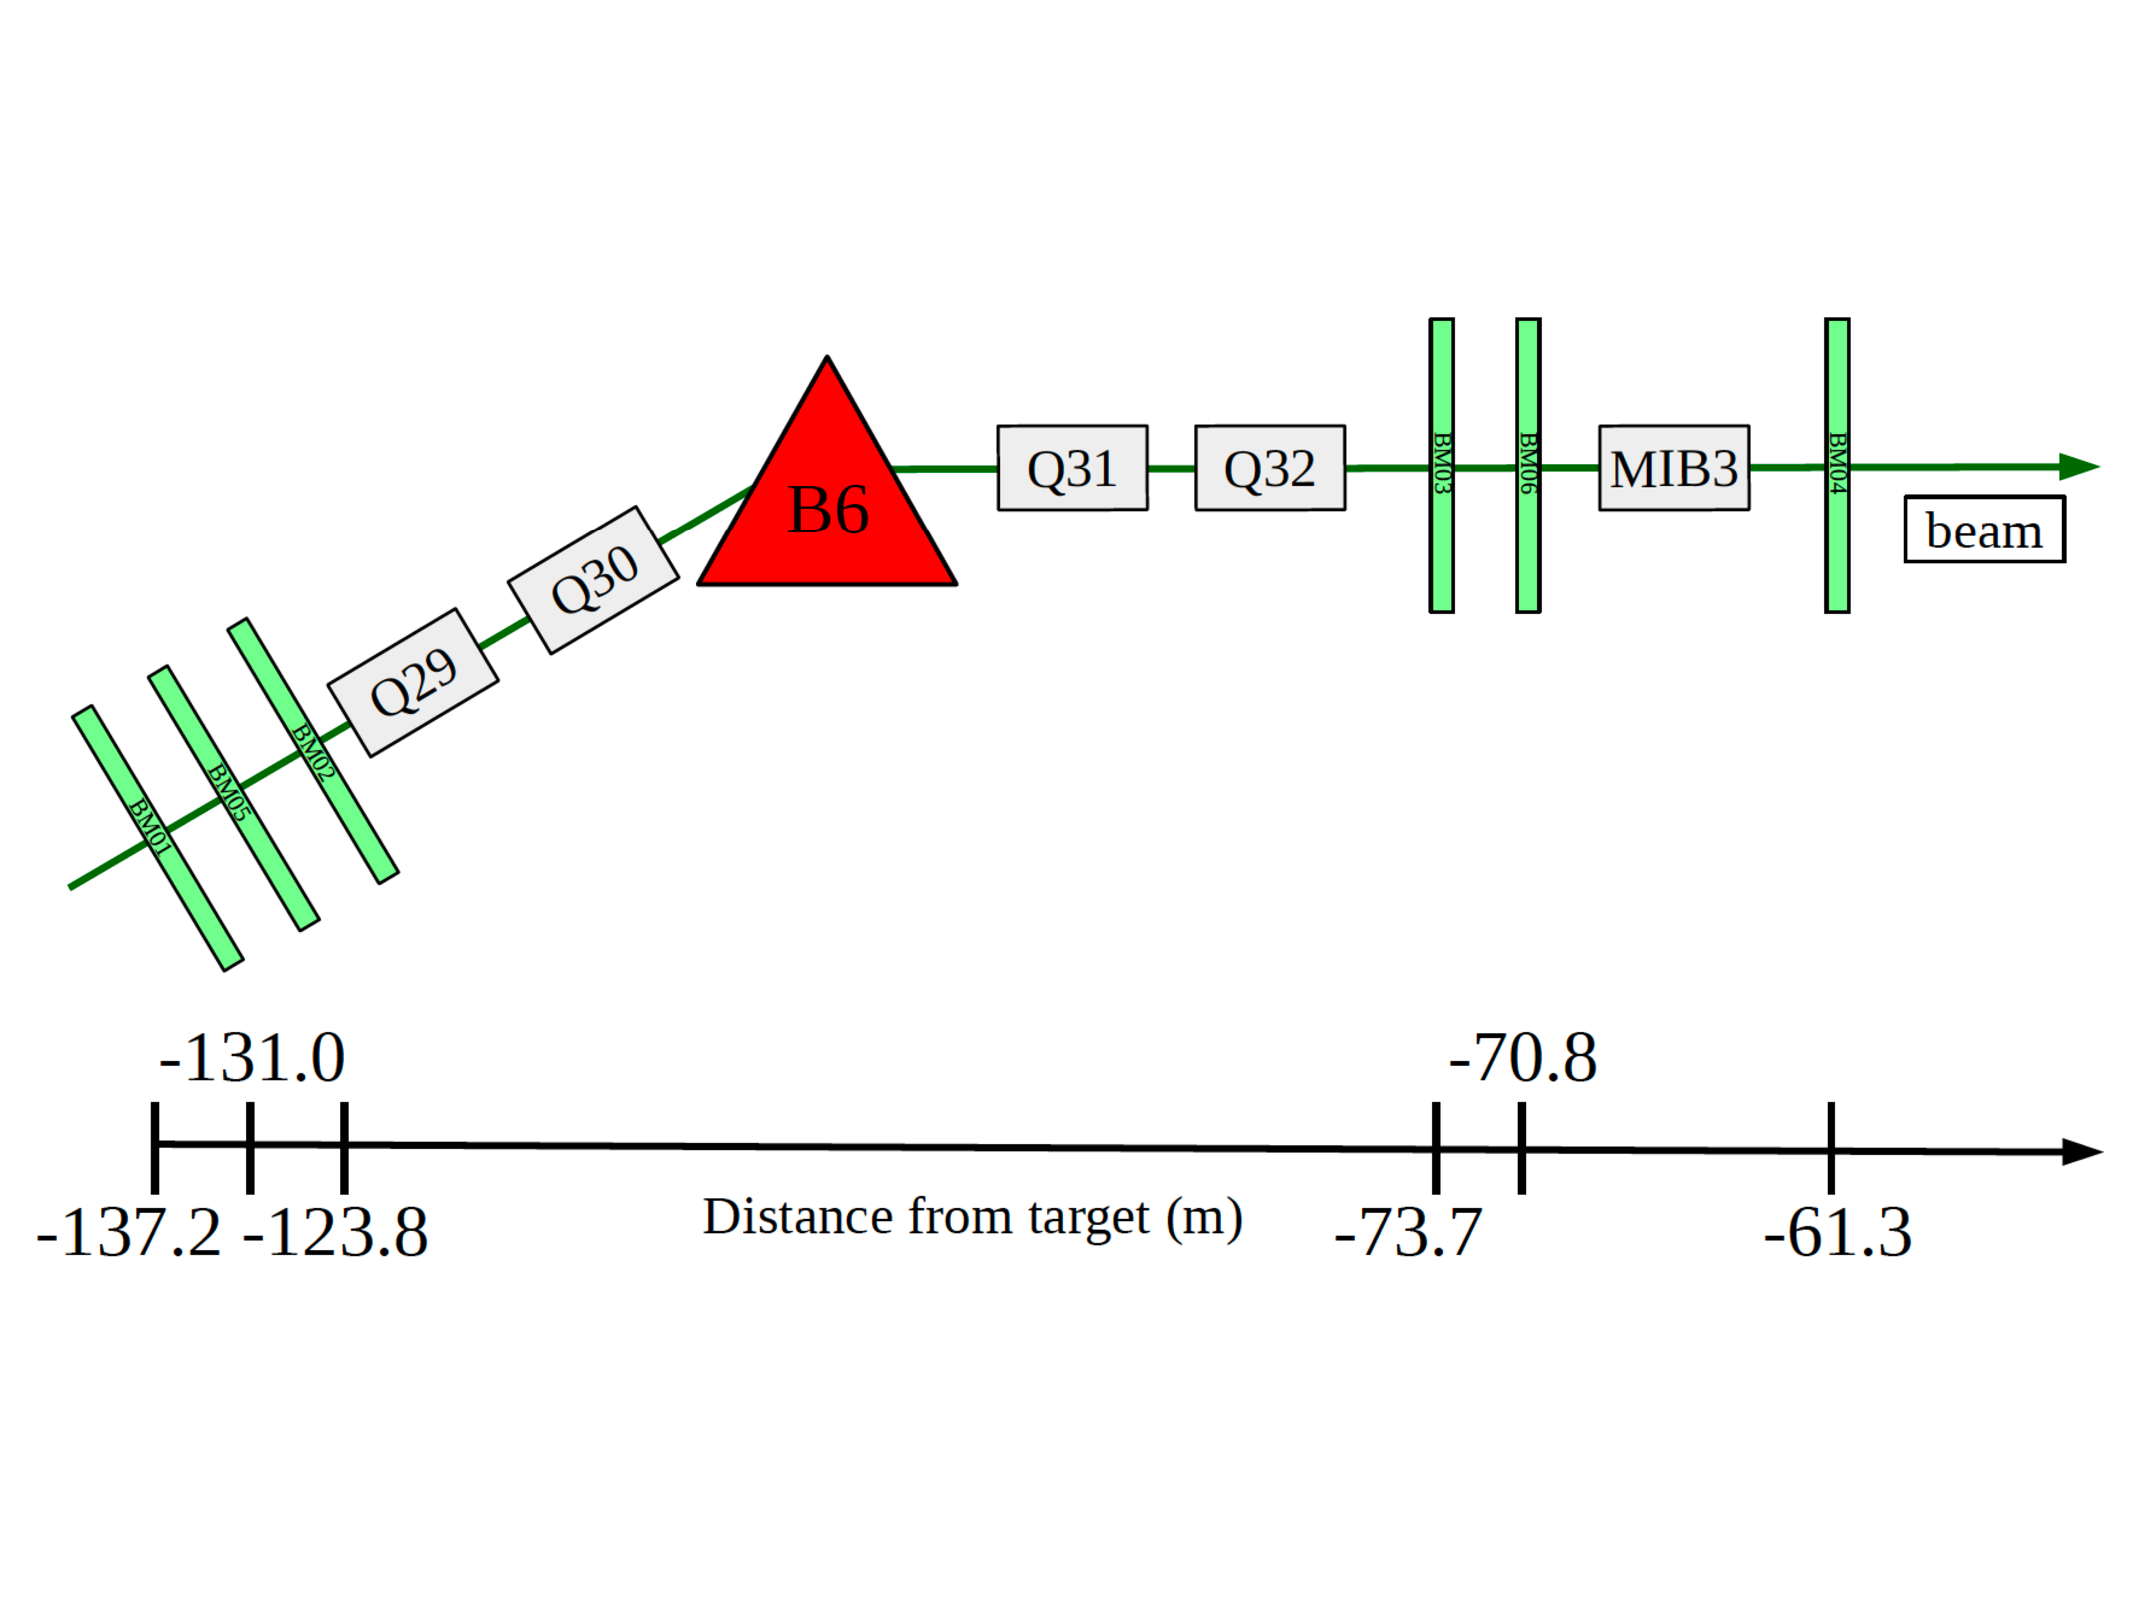
\includegraphics[width=0.8\textwidth]{BeamLine1}
  \caption{Bending the beam to a horizontal position.  The BMS detectors are
    upstream and downstream of the bend 6 magnet.}
  \label{fig::BeamLine1}
\end{figure}

For the 2015 Drell-Yan setup the $\pi^-$ beam intensity was too high for the BMS
station to work properly.  For this reason special low intensity, approximately
10$^6$ s$^{-1}$, $\pi^-$ beams were used in 2014 to determine the momentum
distribution for Drell-Yan data taking.  The beam momentum distribution is shown
in Fig.~\ref{fig::BeamMomBMS} where the average momentum is 190.9~{\gvc} with a
spread of $\pm$ 3.2~{\gvc}. \par

\begin{figure}[h!t]
  \centering
  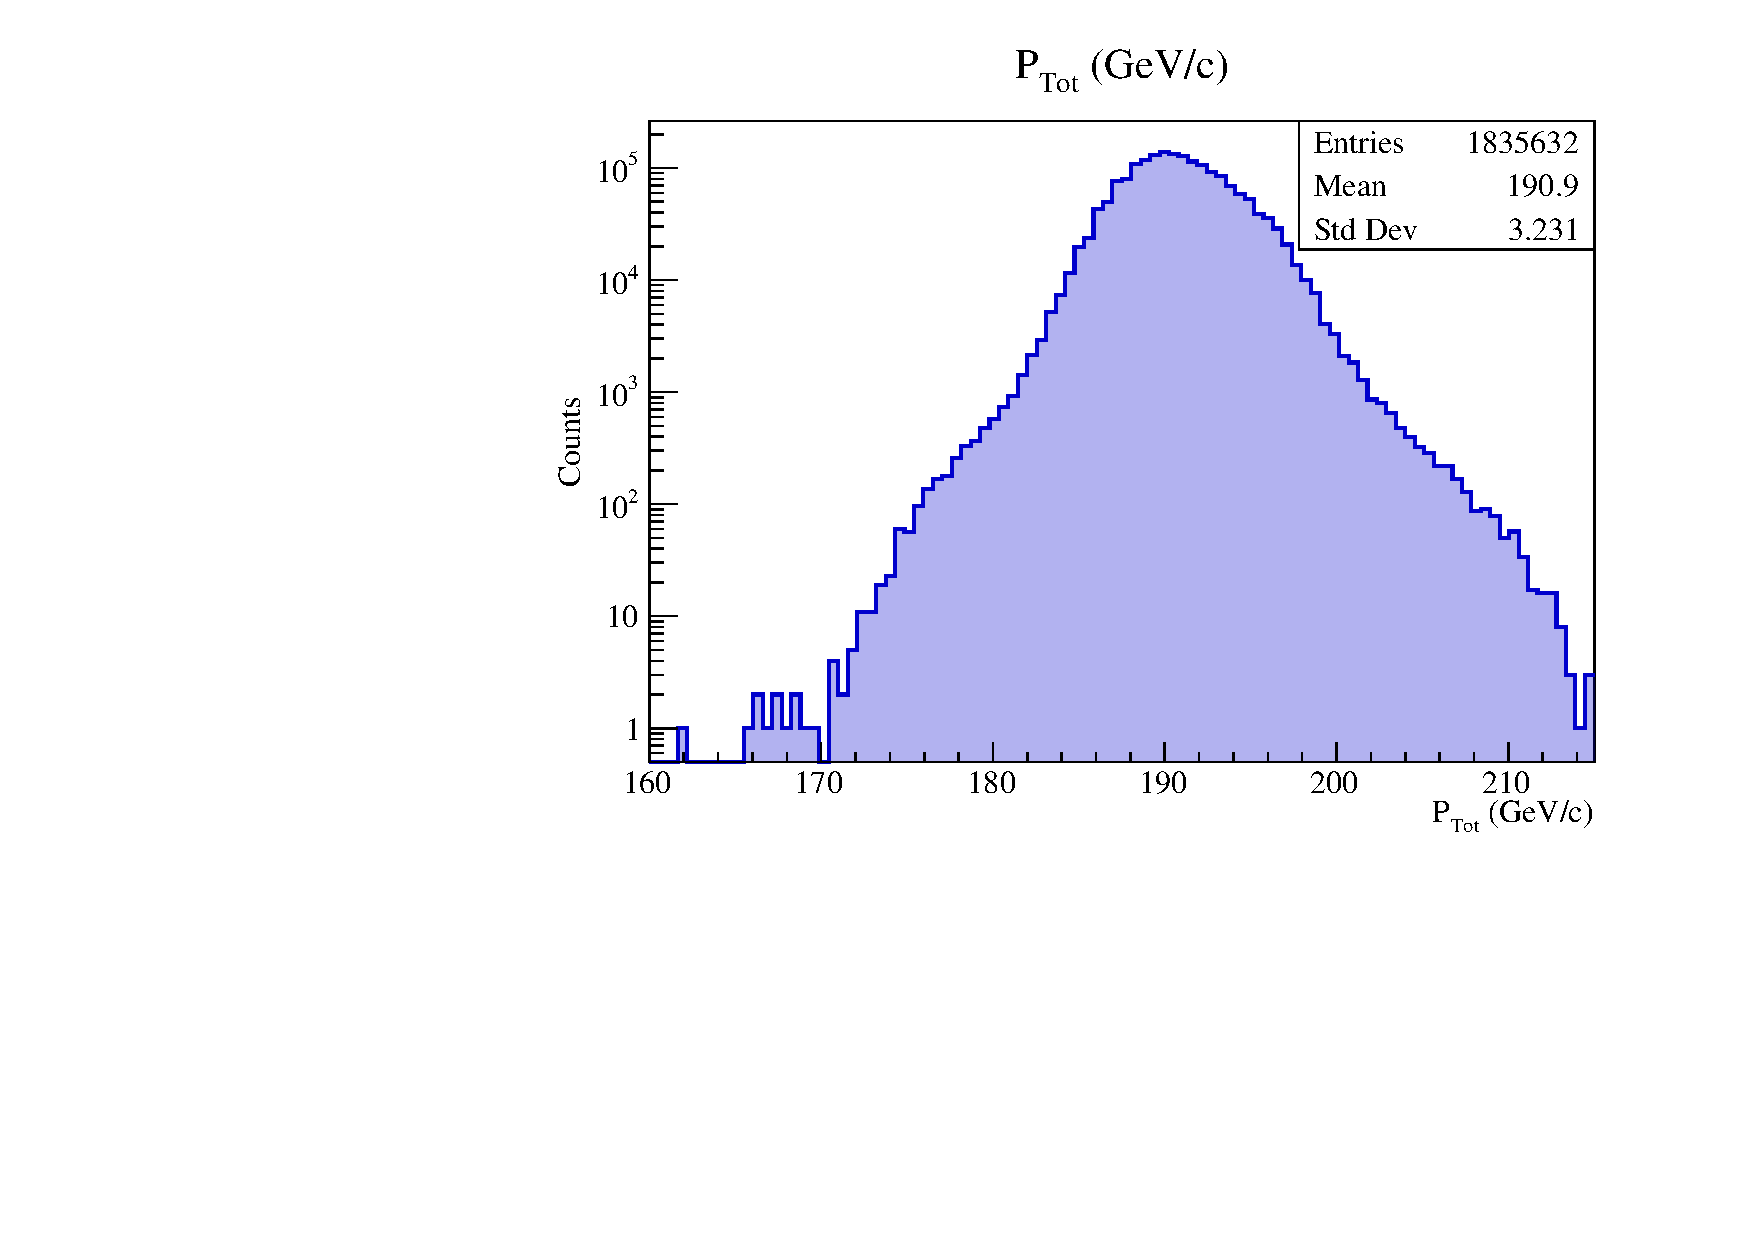
\includegraphics[width=0.5\textwidth]{BeamMomBMS}
  \caption{The momentum distribution of the $\pi^-$ beam, determined during
    dedicated low intensity beam times.}
  \label{fig::BeamMomBMS}
\end{figure}

Approximately 30~m upstream of the target are to two Cherenkov counters (CEDAR)
detectors.  As the hadron beam has contamination from several components these
CEDARs can be used to distinguish between these components.  The CEDARs at
COMPASS are high pressure detectors and have been demonstrated to achieve fast
particle identification for particle momentums up to 300~{\gvc}.  The general
principle of operation for the CEDARs is that two particles with the same
momentum but different mass will emit Cherenkov radiation at different angles
relative to there momentum.  When a particle is traveling faster than the speed
of light in a given medium it emits Cherenkov radiation in a cone centered along
its momentum axis.  The faster the particle is traveling the narrower the angle
of the Cherenkov light cone.  A schematic of the CEDAR operating principle is
shown in Fig.~\ref{fig::cedars}.  In 2015 the CEDARs were measured to be largely
inefficient due to the high beam intensity.

\begin{figure}[h!t]
  \centering
  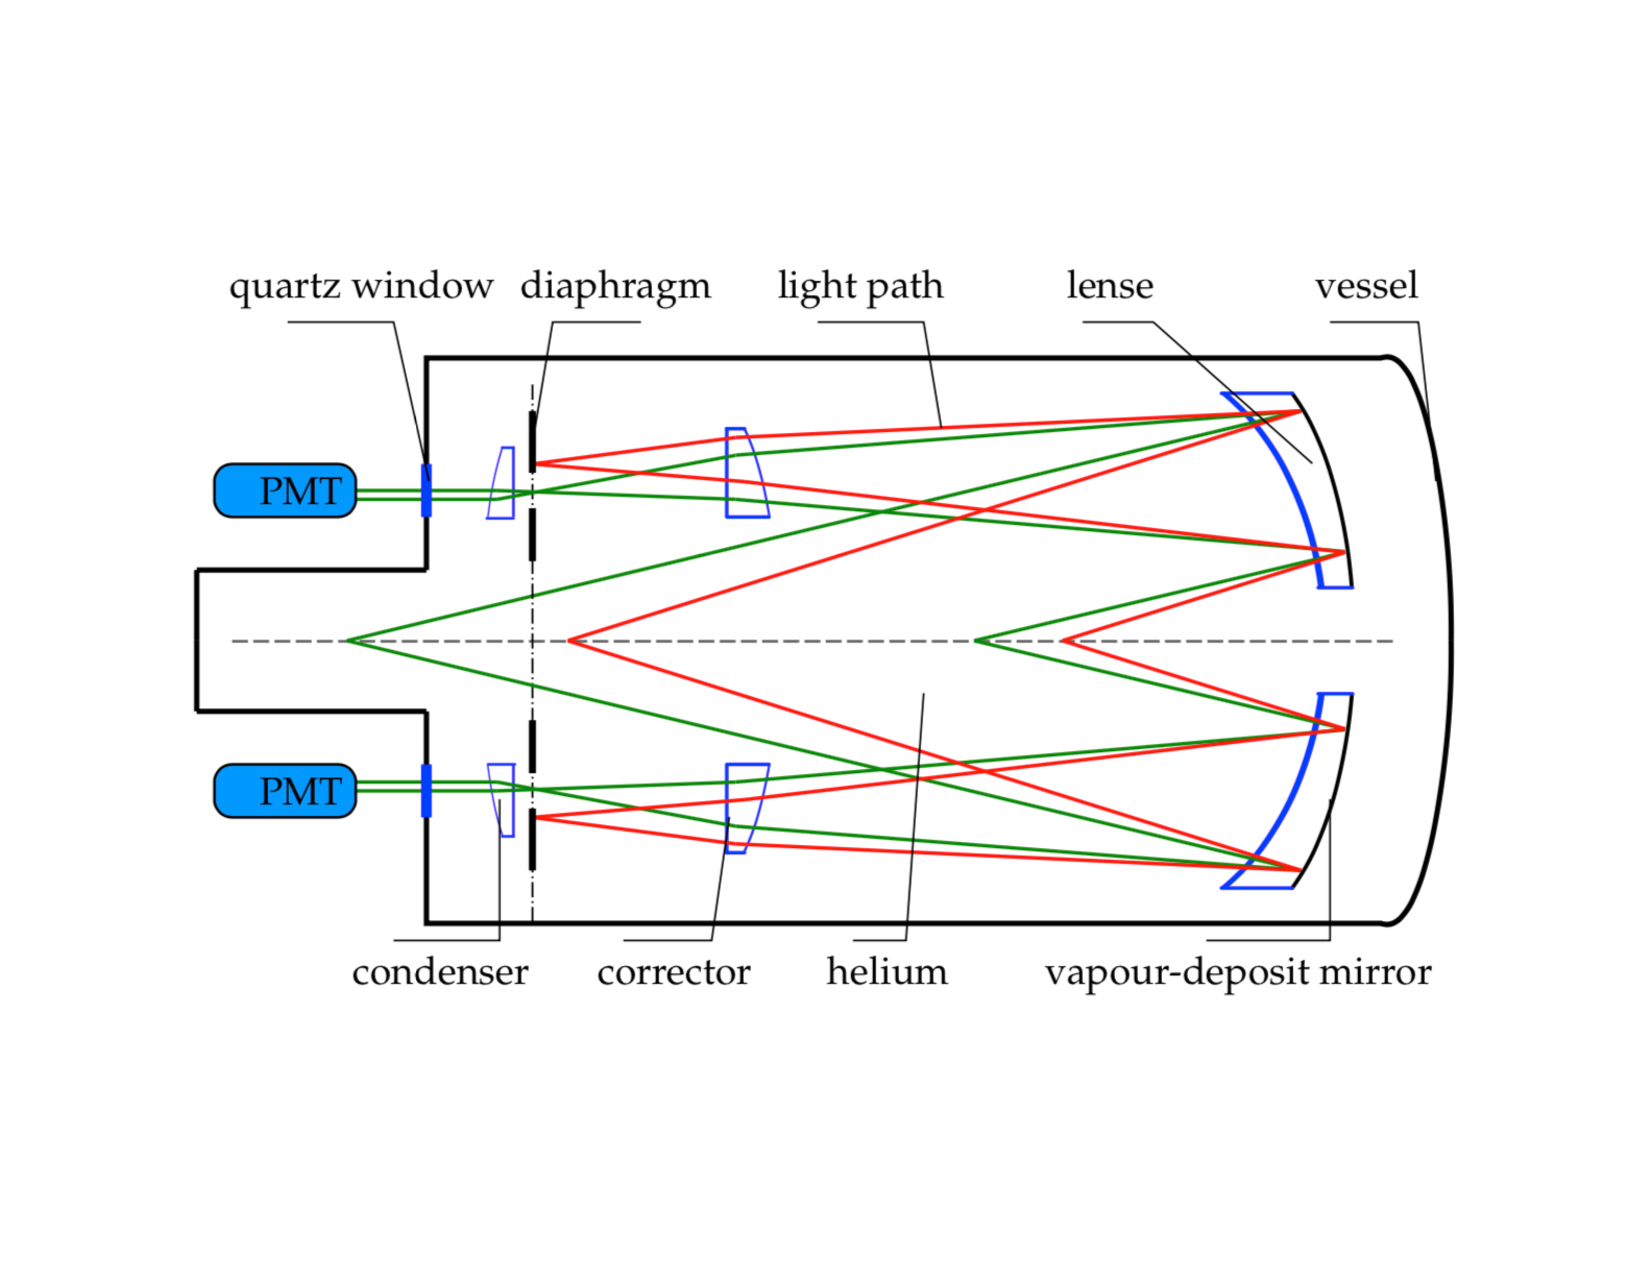
\includegraphics[width=0.5\textwidth,trim=2cm 4cm 2cm 4cm,clip]{cedars}
  \caption{General principles of operation for the CEDARs at COMPASS.  The
    red(green) lines correspond to Cherenkov light emitted from a particle.}
  \label{fig::cedars}
\end{figure}



For years with a transversely polarized target, such as 2015, a chicane system
of dipole magnets is setup in front of the target.  This is because a beam
hitting the target without any angle would then be deflected inside the target
to the left or right of the spectrometer.  For this reason the chicane gives the
beam an angle before hitting the target such that the non-interacting beam exits
the target traveling straight towards the spectrometer.


\section{The Polarized Target}
The polarized target at COMPASS is the most complicated and essential component
of the spectrometer.  It is located upstream of the tracking detectors and
spectrometer magnets and downstream of the beam telescope, described in
section~\ref{sec::tracking}, detectors.  The target consists of 2 or 3
cylindrical cells and the possible materials are either solid state ammonia
(NH$_3$) or deuterated lithium ($^6$LiD) or liquid hydrogen. Fig.~\ref{fig::PT}
shows a schematic of the target.  \par

\begin{figure}[h!t]
  \centering
  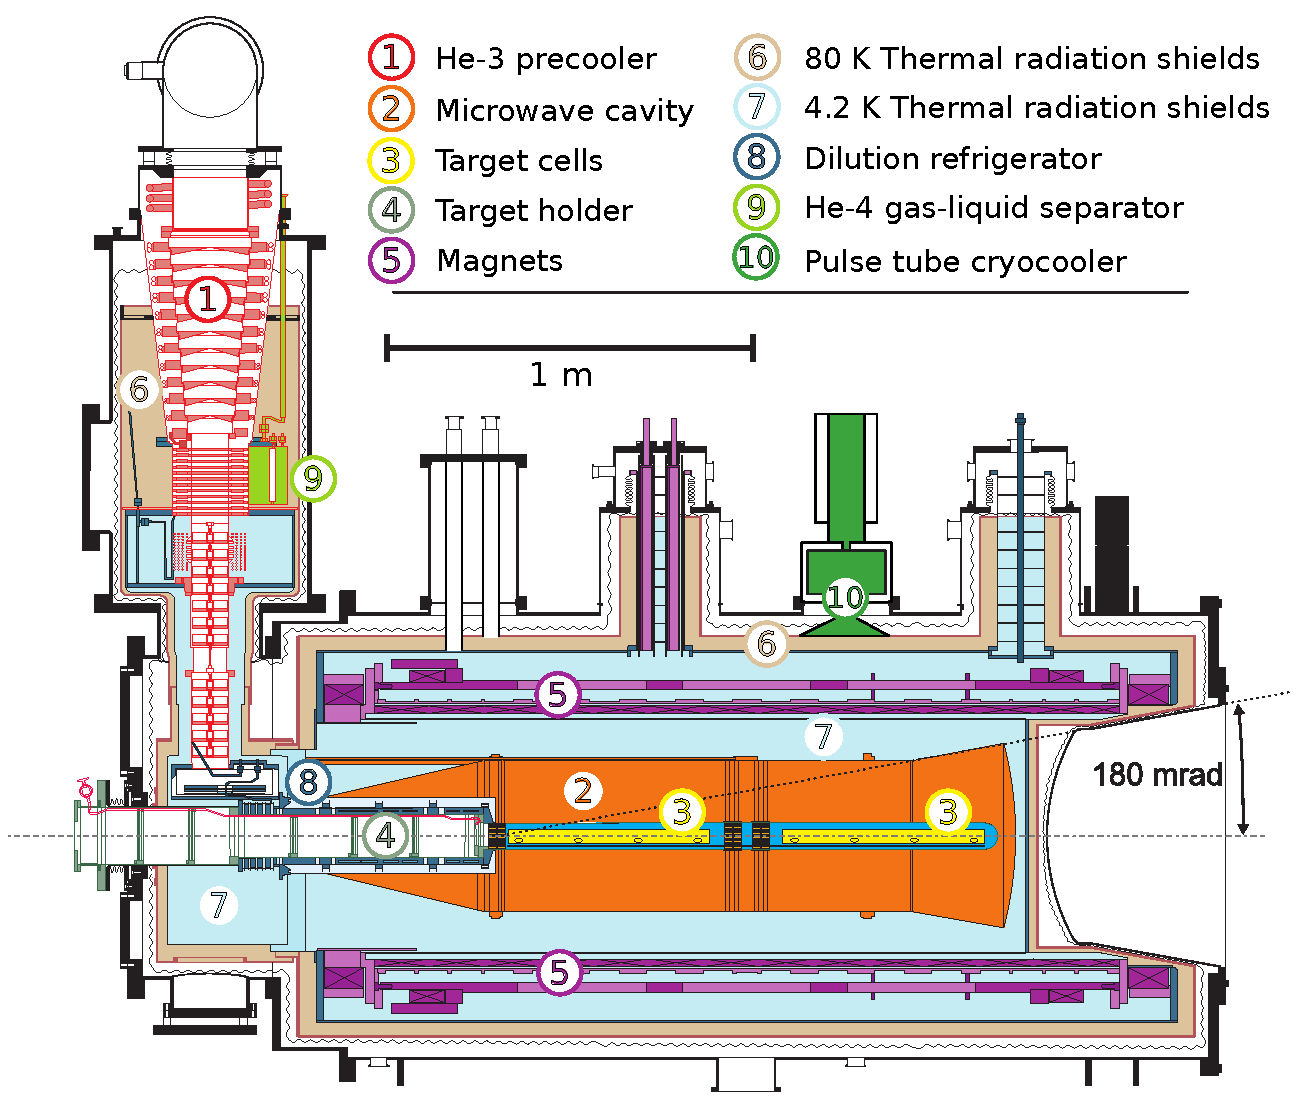
\includegraphics[width=0.8\textwidth]{PT}
  \caption{The polarized target at COMPASS}
  \label{fig::PT}
\end{figure}

Surrounding the cylindrical cells is a longitudinal super conducting magnet
capable of reaching a magnetic field of 2.5T.  This longitudinal magnet
polarizes the target in the direction of the beam momentum and the target
polarization is maintained by keeping the target in a liquid helium bath of
approximately 60mK.  This is called frozen spin mode where the temperature is
maintained by a dilution refrigerator. \par

The target is polarized through the dynamic nuclear polarization (DNP)
method~\cite{DNPmethod}.  This process works by first polarizing electrons in
the target with the longitudinal magnet in the same longitudinal direction for
all target cells while sending electromagnetic radiation in the microwave
spectrum into the target.  Due to their much lower mass, electrons have a larger
magnetic moment and therefore can be polarized at a much faster rate than
protons or neutrons.  For atoms which have a nuclear spin it is then possible
for these atoms to absorb a microwave going to an excited state with the
electron spin anti-parallel to the magnet and the nuclear spin either parallel
or anti-parallel to the magnet depending on the microwave frequency.  The
electron with the anti-aligned spin will then quickly have its spin realigned
while the nucleon will take much longer to lose its polarization due to its
smaller magnetic moment.  This process can continue in this way resulting in a
net nuclear polarization.  Using the DNP method the target can achieve a
polarization of approximately 90\% in three days. \par

The target also includes a 0.63T transverse dipole magnet to change from
longitudinal polarization to transversely polarized.  The target must first be
longitudinally polarized before the transverse target magnet can change the
polarization direction.  Once the target is transversely polarized, the target
polarization can no longer be increased as microwaves can no longer shine on the
target in the polarization direction.  Therefore the polarization will decrease
exponentially.  In 2015 the target was polarized for about half a day between
data taking sub-periods and achieved and average polarization of 0.73\% which
includes the effect of exponential polarization lose with time.  The target
transverse polarization relaxation time was about 1000 hours in 2015. \par

The target polarization was measured with 10 NMR coils while in longitudinal
magnet mode.  In the 2015, each target cell had the most upstream and downstream
coils in the center of the target cell and the other three coils on the outside
perimeter of the target cells.  Due to the fact that the polarization can only
be measured with the longitudinal magnet on, the polarization is only measure at
the start and finish of a transversely polarized data taking.  The intermediate
polarization are then determined by exponential interpolating between these two
times.

In 2015 the setup was two transversely polarized target cells of 55~cm length
and 2~cm in radius, separated by 20~cm and oppositely polarized.  The
polarization of the target cells was flipped ever two weeks of data taking to
reduce systematic effects.  Due to the fact that the beam needs to be precisely
steered onto the target anytime a beam line magnet is changed and that the
chicane magnets upstream of the target are setup for only one transverse target
direction, the transverse target magnet only pointed downward in 2015.  To
achieve a polarization flip the target polarization had to therefore be rotated
back to the longitudinal direction and the input microwaves had to be changed to
achieve the desired polarization direction. \par

The target material in 2015 was NH$_3$ where the protons in the three hydrogen
atoms were the only nucleons with nuclear spin.  Therefore only some fraction of
the target was able to be polarized and one would expect that this fraction is
3/17.  However to get a more accurate determination of the dilution factor the
follow calculation was used
\begin{equation}
  f = \frac{n_H\sigma^{DY}_{\pi^-H}}
  {n_h\sigma^{DY}_{\pi^-H} + \sum_A n_A\sigma^{DY}_{\pi^-A}},
\end{equation}
where $f$ is the dilution factor, $n_H$ is the number of hydrogen atoms in
NH$_3$, $n_A$ is the number of other nucleons in NH$_3$, and
$\sigma^{DY}_{\pi^-H}$ and $\sigma^{DY}_{\pi^-A}$ are the Drell-Yan
cross-section for pion hydrogen scatter and pion nucleon scattering
respectively.  The cross-section were determined using a parton-level
Monte-Carlo program MCFM~\cite{MCFM}.  The dilution factor was also further
scaled down by studies of reconstruction migration between target cells.  The
average dilution factor in 2015 was 0.18.


\section{Tracking Detectors} \label{sec::tracking}
The goal of the tracking detectors is to determine a point in space where a
particle traversed.  The COMPASS tracking detectors attempt to do this for a
wide range of angles, momentums and at different rates.  For these reason there
are several planar tracking technologies used at COMPASS which can be divided
into three categories: very small angle tracker, small angle trackers and large
area trackers.  As the name suggest very small angle trackers measure tracks
with small angle deflections from the beam axis which are essentially beam
particles.  The small area trackers measure particle tracks with low but
non-zero angle have central dead zones.  The large area trackers are several
meters in height and width and measures the largest deflection angles up to
180~mrad. \par

All of these trackers are split into stations where each station corresponds to
several detectors at roughly the same z-position along the beam line.  Each
station measures a track position in one or more orientation while most measure
tracks in three or more orientations.  The coordinate orientations measured are
the X and Y coordinates which are the horizontal and vertical directions
respectfully and as well the U and V coordinates which are rotated at different
angles with respect the X and Y coordinates. \par

\subsection{Very Small Angle Trackers}
The very small angle trackers extend up to 3~cm away from the beam axis.  This
is the region with the highest number of tracking particles and therefore these
detectors must be able to handle the highest rates up to 5x10$^7$~Hz.  The two
detector types that make up the very small angle trackers are either
scintillating fiber detectors (SciFi) or silicon microstrip detectors.  These
two detector types are complementary to each other as the former have very good
timing resolution while the latter have very good spacial resolution. \par

There are three silicon stations possible at COMPASS with active detecting areas
of 5x7~cm$^2$.  The spacial resolution of these detectors is nominally 10~$\mu$m
and the timing resolution is nominally 2.5~ns.  For the 2015 setup, the beam
intensity was too high for the silicon detectors to operate and therefore these
detectors were not used in 2015. \par

There are 10 SciFi stations available at COMPASS with sizes varying from
3.9x3.9~cm$^2$ to 12.3x12.3~cm$^2$ planar areas.  The fiber diameters vary
between detectors and are 0.5~nm, 0.75~nm and 1~nm.  Several fibers are bundled
together to determine a strip hit position and the resulting nominal spacial
resolutions are 130~$\mu$m, 170~$\mu$m and 210~$\mu$m.  The nominal timing
resolution of these detectors about 400~ps.  In 2015 three SciFi stations made
up the beam telescope and were placed upstream of the target to measure the beam
trajectory and timing information.  A fourth SciFi station was place in the LAS
section of the spectrometer. \par

\subsection{Small Angle Trackers} \label{sec::SAT}
The small angle trackers are small area detectors that detect particles with a
non-zero defection angle.  They cover 5~cm to 40~cm from the beam axis where the
rate drops two orders of magnitude relative to the very small angle trackers to
approximate 10$^5$~Hz.  At COMPASS there are two types of small area tracking
detectors: micromesh gaseous structure (micromegas) and gas electron multipliers
(GEMs). \par

There are three micromega stations at COMPASS all location sequentially after
each other between the target and the first spectrometer magnet.  All three
detectors measure four coordinate projections and have an active area of
40x40~cm$^2$ with a 5~cm diameter dead zone.  The micromegas operate by having a
conversion region and a smaller amplification region.  An ionized particle
produced in the conversion region will drift through an electric field too small
for amplifaction of around 3.2~kV/cm to the amplification region where the
electric field is around 50~kV/cm and is high enough to amplify the sign which
is then read out on strips.  The conversion and amplification regions are
separated by a metallic micromesh material.  The electrons pass through the
micromesh without resistance and are not rimmed out.  The micromegas have good
spacial resolution because the thickness of the amplification region is only
100~$\mu$m which is small enough to prevent the electron avalanche from
spreading out much transversely between strips.  The separation of the larger
conversion region from the smaller amplification region with the micromesh
prevents electric field lines from being distorted in the conversion region and
therefore prevents the primary electrons from drifting slower in the conversion
region.  This allows micromegas to operate at a higher rate than would be
possible otherwise.  This principle of operation is illustrated in
Fig.~\ref{fig::MicroMega}.  The strips in the central part of the detector are
360~$\mu$m corresponding to a resolution of about 100~$\mu$m and the strips in
the outer region are 460~$\mu$m corresponding to a resolution of about
120~$\mu$m.  The nominal timing resolution 9~ns.  In 2015 the micromegas were
upgraded to include a pixelized section covering much of the dead zone
area. \par

\begin{figure}[h!t]
  \centering
  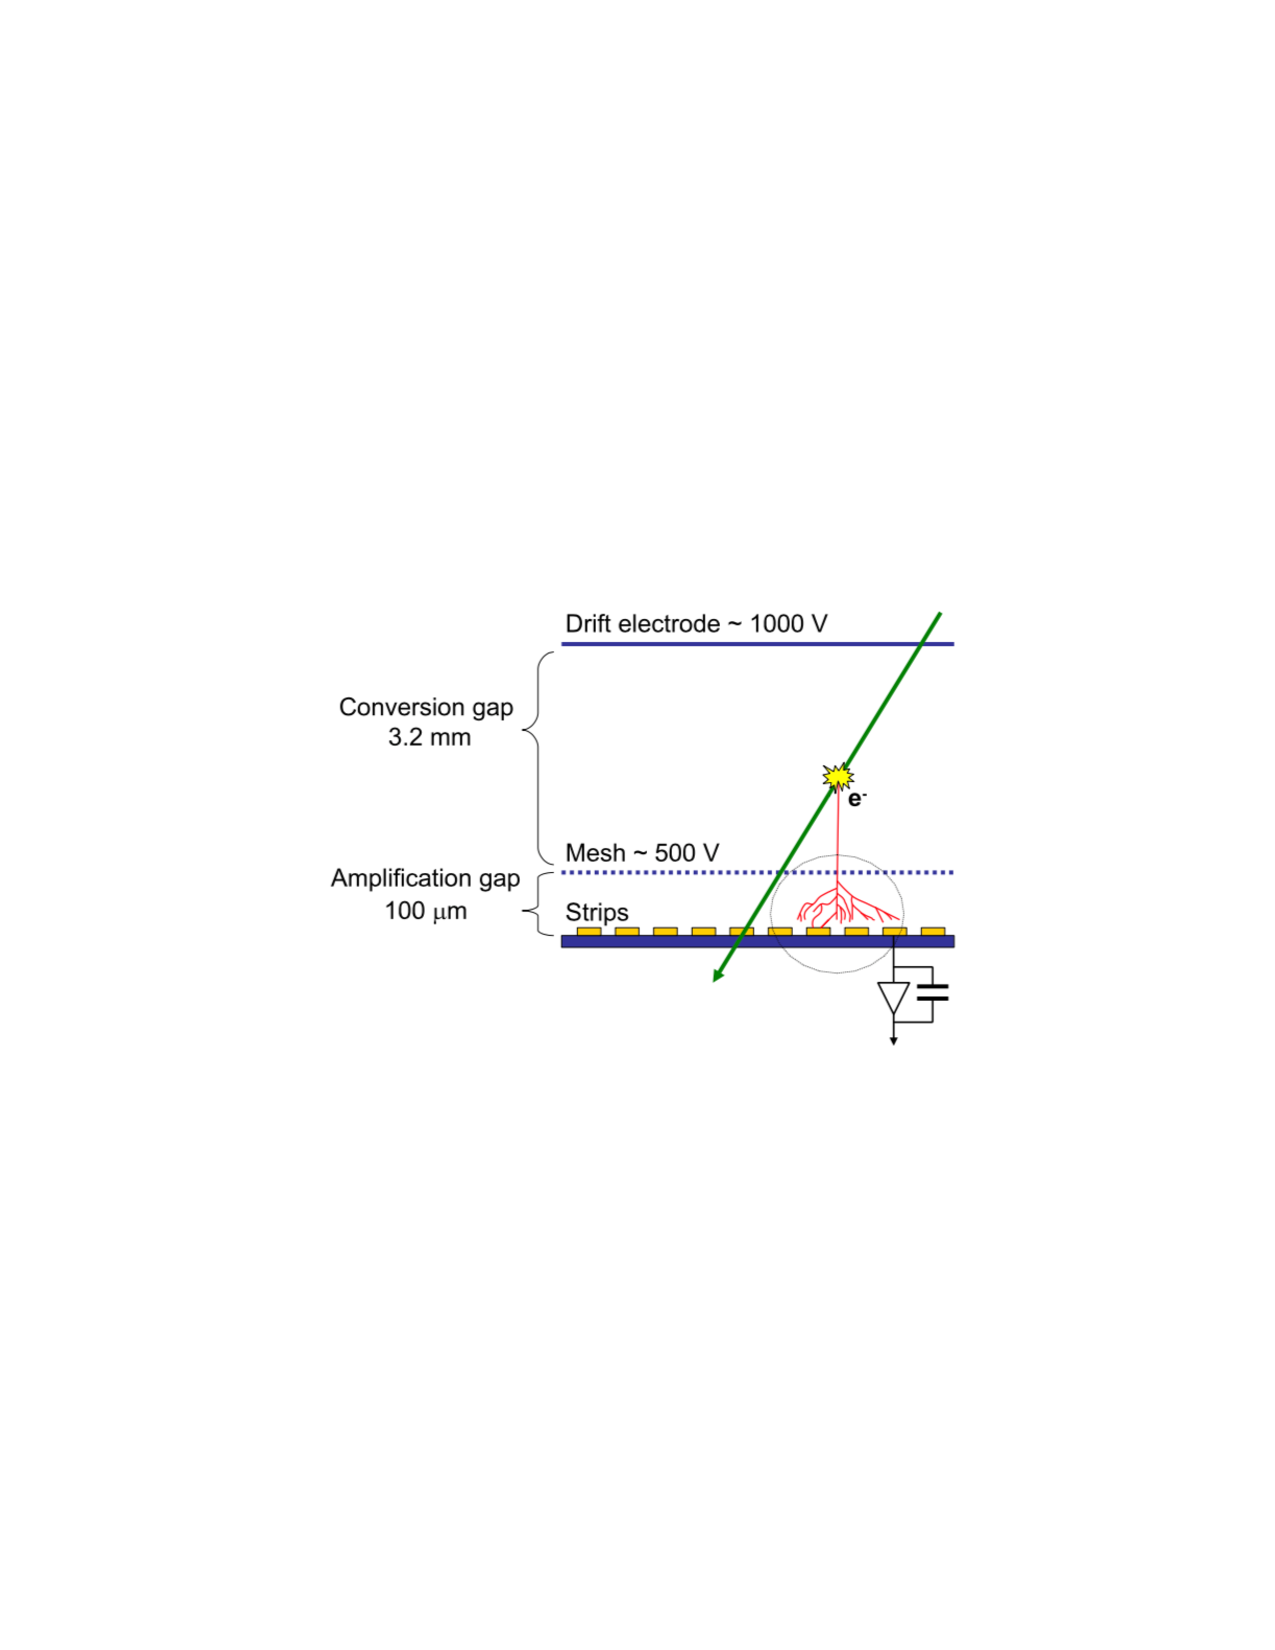
\includegraphics[width=0.7\textwidth, trim=4cm 10cm 4cm 10cm, clip]{MicroMega}
  \caption{Principle of operation for the micromesh gaseous structures
    (micromegas)}
  \label{fig::MicroMega}
\end{figure}

There are eleven GEM detectors located throughout the COMPASS spectrometer
starting after the first spectrometer magnet down to the end of the
spectrometer.  These detectors are close to the beam axis and are mounted on a
large area tracker covering the dead zone region of the large area tracker.  All
eleven detectors have an active area of 31x31~cm$^2$ and a 5~cm diameter dead
zone.  In times of lower beam intensity the dead zones can be turned on as an
active area.  The detector is split into four regions separated by a polymide
foil (50~$\mu$m thick) clad with copper on both sides with around
10$^4$~cm$^{-1}$ drifting holes of 70~$\mu$m diameter.  There in an electric
potential of a few hundred volts between each foil layer.  The GEM detectors
speed up the amplification process by splitting the amplification avalanche into
three locations there by allowing for a higher rate of operation then would
otherwise be possible.  The electron amplification occurs around the holes of
each of the three foil dividers which therefore speeds up the overall drift time
from the ionization location to the strip readout.  This principle of operation
is shown in Fig.~\ref{fig::GEM}.  The nominal timing and spacial resolution of
the GEM detectors is 10~ns and 110~$\mu$m respectively.  Two pixelized GEM
detectors where also in operation but were not as crucial for the 2015 Drell-Yan
measurement.

\begin{figure}[h!t]
  \centering
  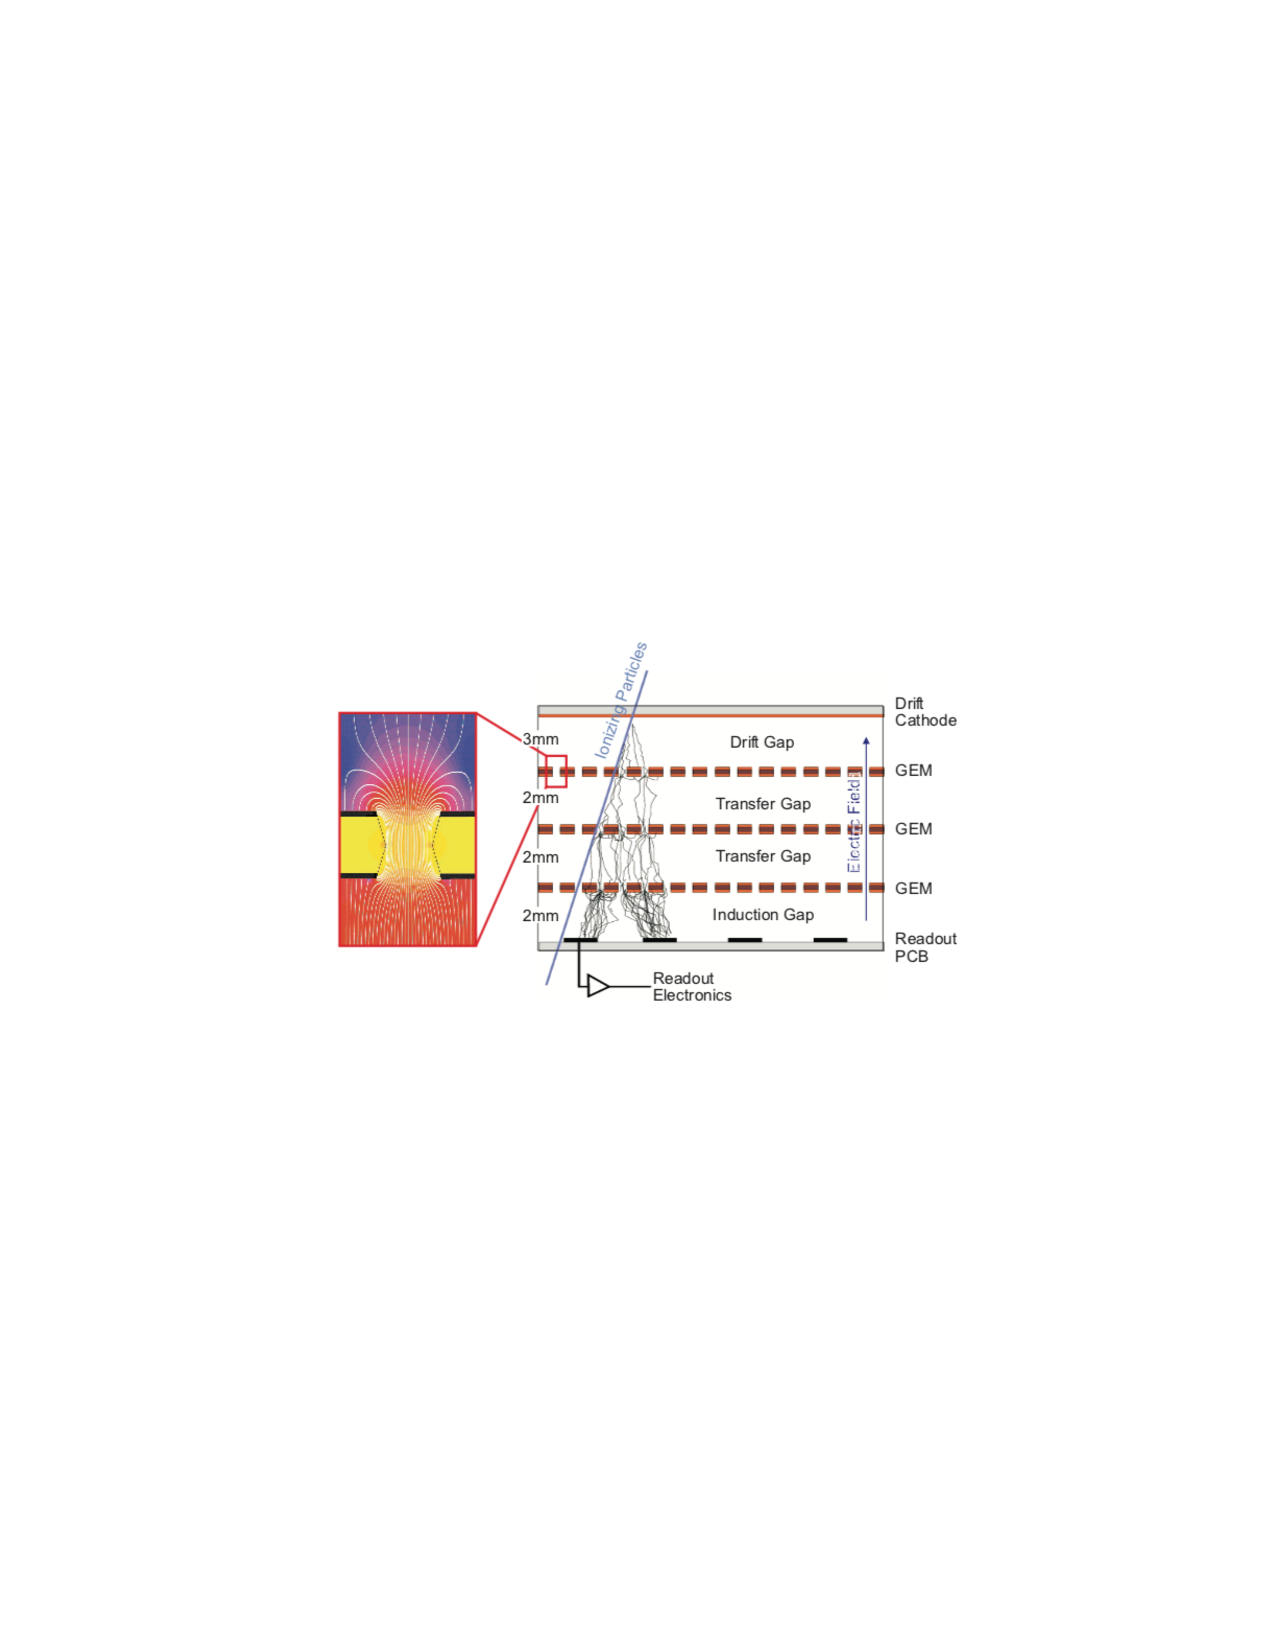
\includegraphics[width=0.7\textwidth,trim=4cm 10cm 4cm 10cm, clip]{GEM}
  \caption{The operation principle of the gas electron multiplier (GEM)
    detectors}
  \label{fig::GEM}
\end{figure}

\subsection{Large Area Trackers}
The large area trackers measure the largest polar scattering angles at COMPASS.
Their dead zones mostly coincide with a small area tracker, described in the
previous section~\ref{sec::SAT}, which therefore means these detectors do not
have to process the higher fluxes very close to the beam line.  The most
important feature of these detectors is that they have a large planar area but
as a consequence their position and timing resolution is not as good as the
small and very small angle trackers.  The types of large area trackers used are
COMPASS are all gaseous detectors and include drift chambers (DCs), straw tube
detectors (straws) and multi-wire proportional chambers (MWPCs). \par

The first four drift chambers downstream of the target are named DC00, DC01,
DC04 and DC05.  The first two, DC00 and DC01, have smaller active areas of
180x127~cm$^2$ and a circular dead zone of 30~cm diameter and are positioned
upstream of the SM1 magnet.  The rates upstream of SM1 are higher due to low
energy particles produce in the target, which are bent out of the acceptance of
spectrometer by SM1.  Therefore DC00 and DC01 need to be able to process a
higher particle flux.  The next two drift chambers, DC04 and DC05, are
downstream of SM1 and both have larger active areas of 240x204~cm$^2$ and as
well have dead zones of 30~cm diameter.  The active areas of all four of these
DCs was roughly chosen to coincide with the acceptance of the SM1 yoke.  DC05
was first installed for the 2015 Drell-Yan data taking and is further described
in chapter~\ref{ch::DC05}.  All four of these DCs measure four projection views
corresponding to eight detector layers.  A sketch of the principle of operation
is shown in Fig.~\ref{fig::DCoperation}.  The nominal spacial resolution for
these detectors is 250~$\mu$m. \par

\begin{figure}[h!t]
  \centering
  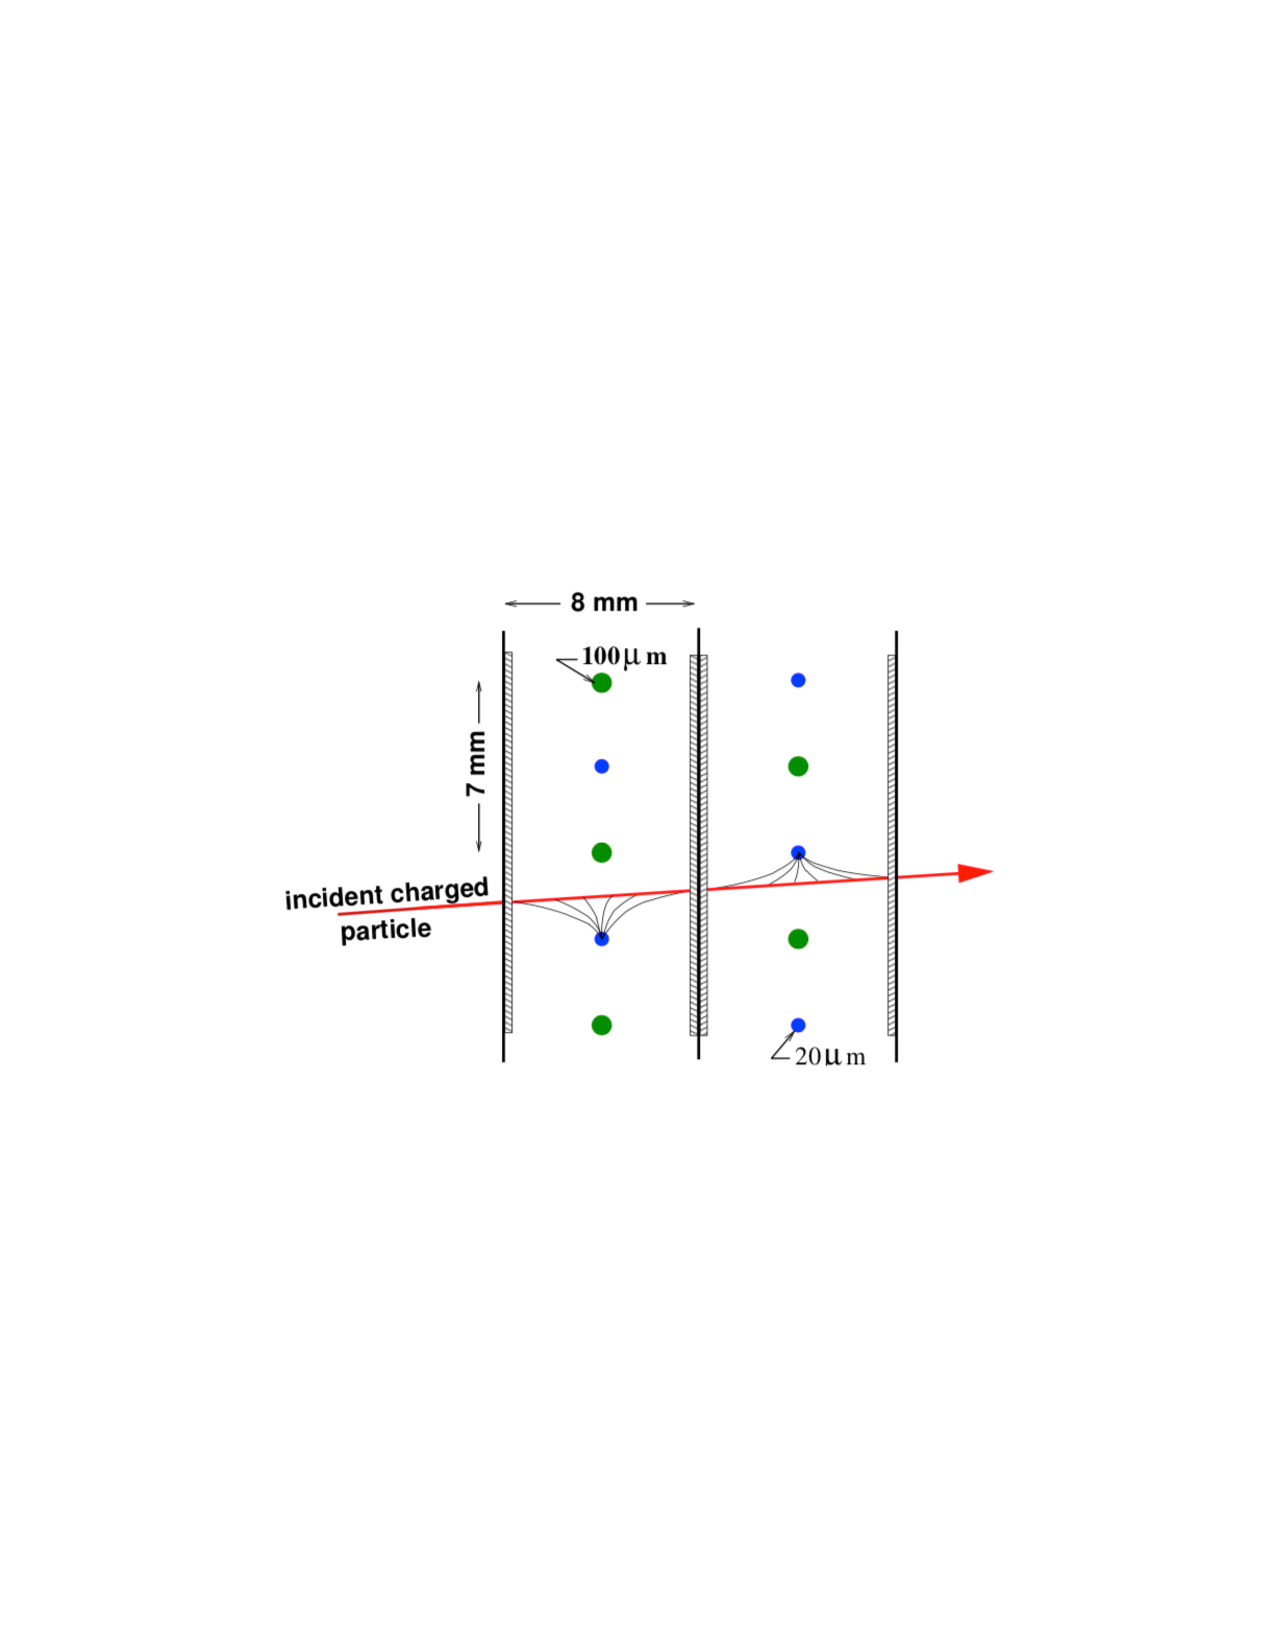
\includegraphics[width=0.6\textwidth,trim=4cm 8cm 4cm 10cm,
    clip=true]{DCoperation}
  \caption{Drift cell of a Drift chamber with the ionized drift electron lines
    coming from the incident charged particle}
  \label{fig::DCoperation}
\end{figure}

There are additional drift chambers downstream of the SM2 magnet, named W45.
W45 consist of six detector stations which each have an active area of
520x260~cm$^2$ and a circular dead zone of 50~cm or 100~cm diameter.  Each W45
station measure two projection views corresponding to four detector layers.  The
drift cells in W45 are 40x10~mm$^2$ and the spacial resolution is nominally
1500~$\mu$m. \par

In 2015 there were two straw stations in operation named ST03 and ST05.  ST03
was in the large angle spectrometer after DC05 and consisted of two stations
measuring six projection views.  ST05 was in the small angle spectrometer and
measured three projection views.  The active areas of horizontal wire stations
is 350x243~cm$^2$ and the active area of the rotated wires is 323x272~cm$^2$.
The principle of operation for the straw detectors is very similar to that of a
drift chamber however instead of having the detector made up of connected drift
cells the straw detectors are made of circular tubes.  Each tube consist of a
gold plated tungsten anode wire in the center and the walls of the tube make up
a cathode.  Due to the fact that the cathode completely surrounds the anode wire
there is no electrical interference between neighboring anode wires as there is
for drift chambers.  For this reason the electric field in each tube is easier
to control and the ionized electron drift speed is more linear than other
detectors.  Each straw detector plane is divided into sections where the straw
tubes in the outer most section from the beam line have a diameter of 9.6~mm and
the tubes close to the beam line have a diameter of 6.1~mm.  In additional in
the central part of the detector there is a physical hole dead zone of
20x20~cm$^2$.  The nominal position resolution for these detectors is 400~$\mu$m
and a frontal schematic is shown in Fig.~\ref{fig::frontalStraw}.  For the
reason that most of the final state muon are reconstructed in the large angle
spectrometer and the fact that many of the high voltage modules were not
operation for ST05 in 2015, ST05 was not used for track reconstruction for
Drell-Yan data. \par

\begin{figure}[h!t]
  \centering
  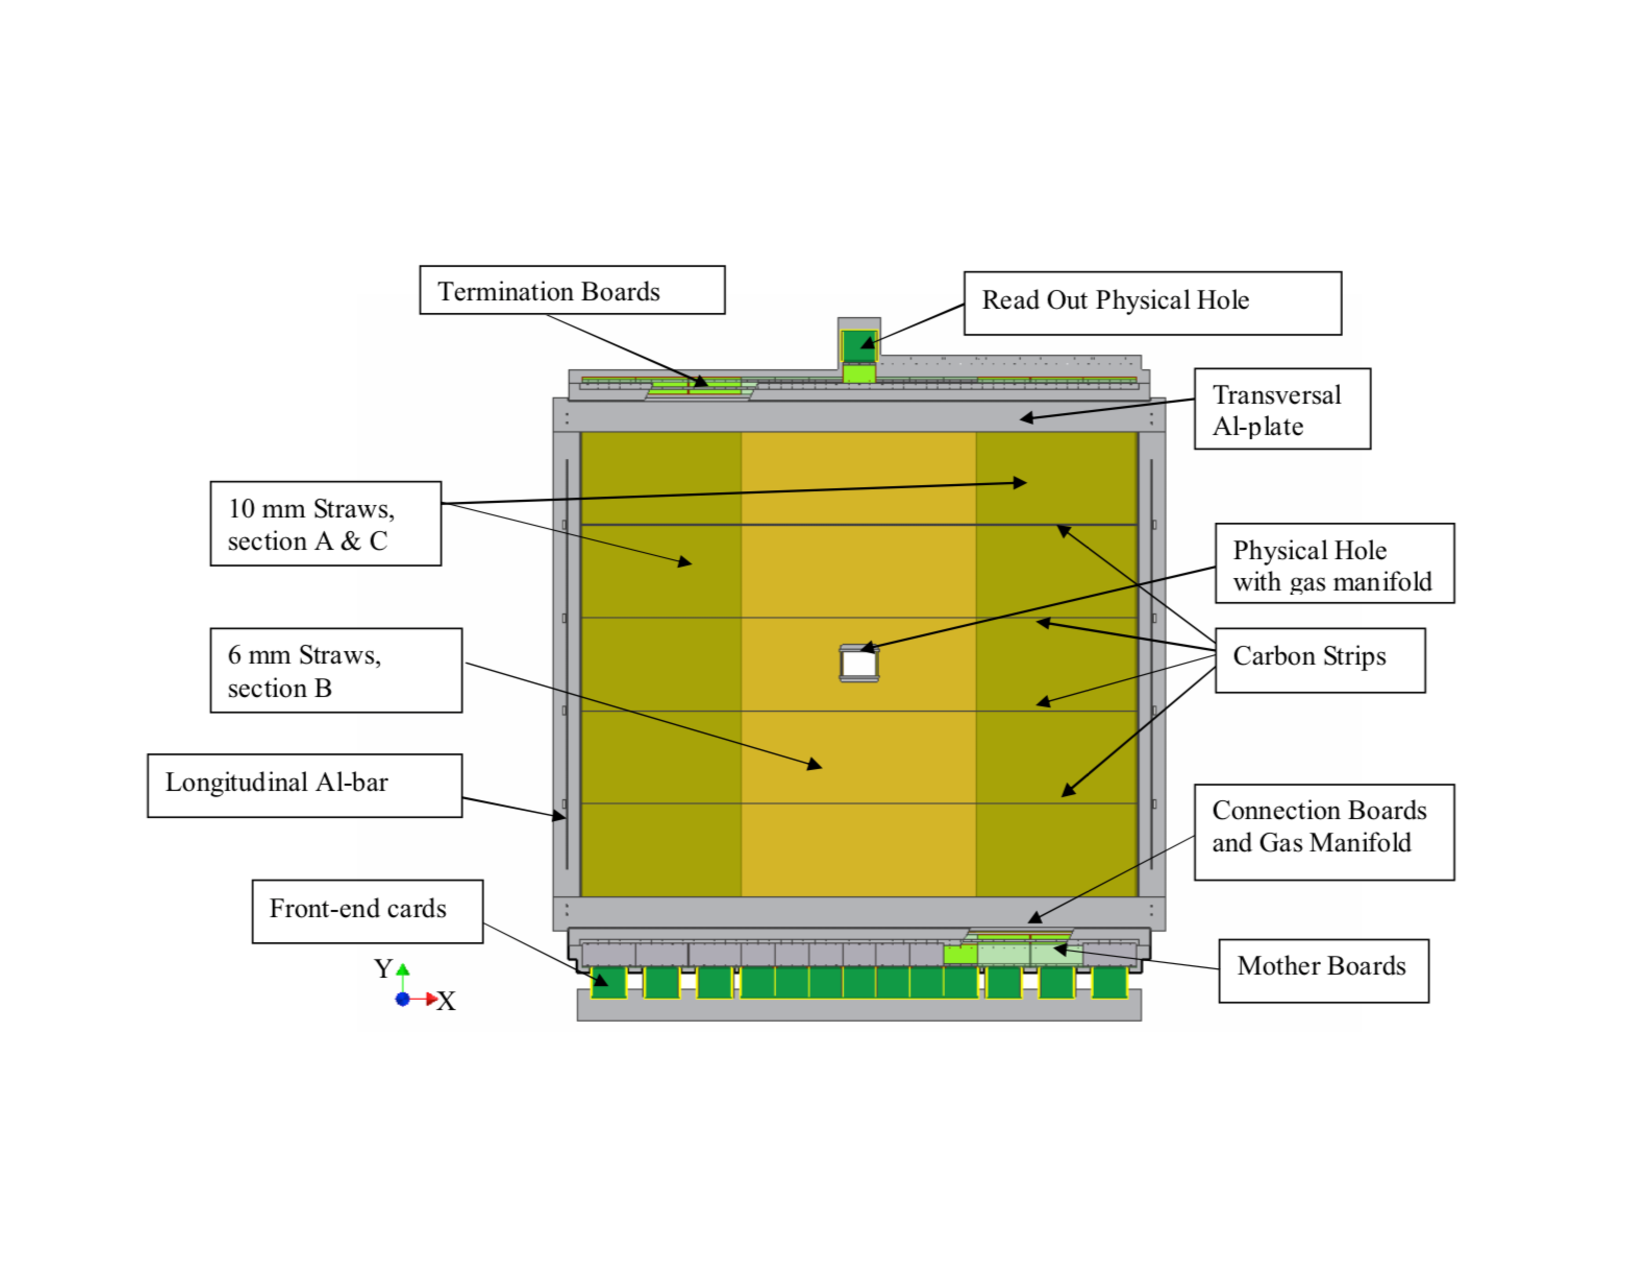
\includegraphics[width=0.8\textwidth,trim=2cm 4cm 3cm 4cm,clip]{frontalStraw}
  \caption{Front on view of a the active area of a straw detector at COMPASS}
  \label{fig::frontalStraw}
\end{figure}

Another large area tracker that operates similarly to the straw tube detectors
is the richwall detector.  This detector is located before the SM2 magnet and
after ST03 with an active area of 5.27x3.91~cm$^2$ and a central dead zone of
1.02x0.51~cm$^2$.  The detector consist of eight layers of mini drift tubes
(MDT) shown in Fig.~\ref{fig::richwallMDT}.  The central part of each MDT
includes a gold plated tungsten sense wire.  The nominal position resolution of
this detector is 600~$\mu$m. \par

\begin{figure}[h!t]
  \centering
  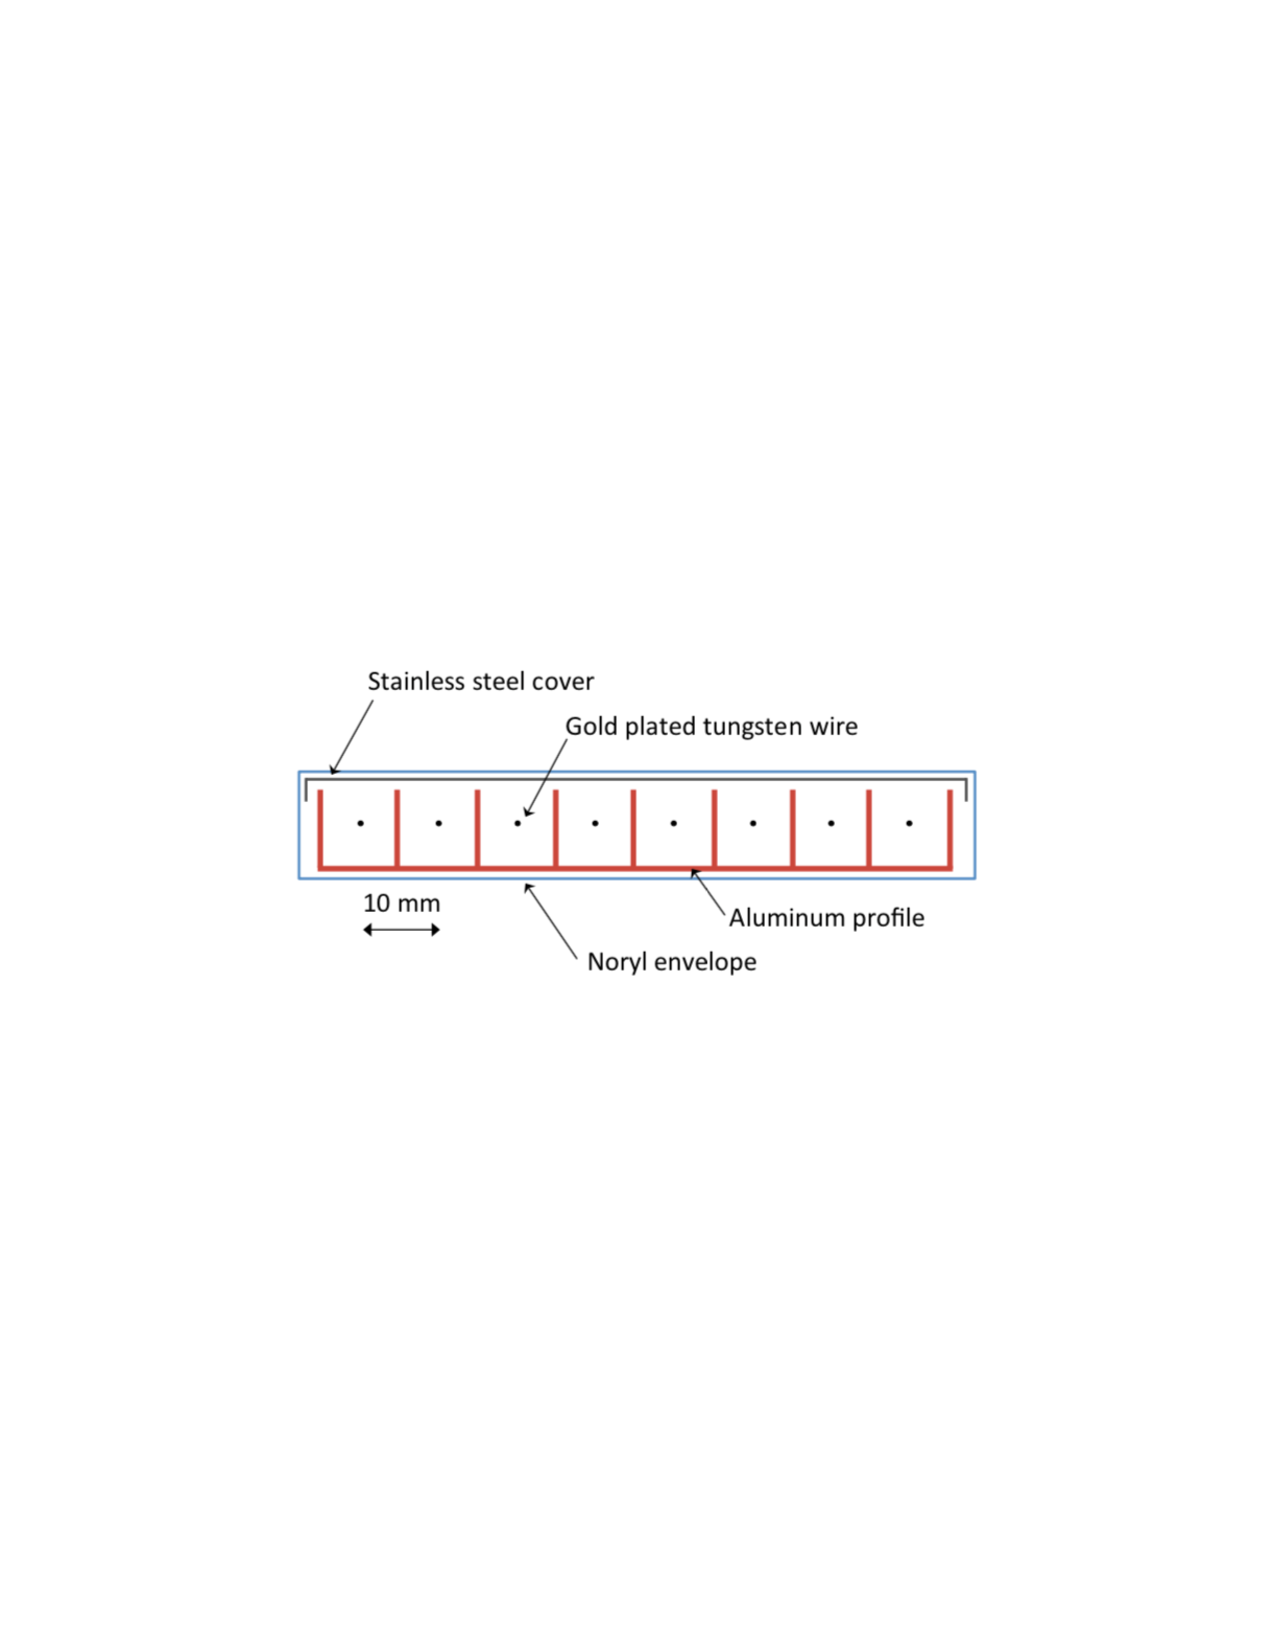
\includegraphics[width=0.45\textwidth, trim=5cm 12cm 5cm 10cm, clip]
                  {richwallMDT}
  \caption{The richwall mini drift tubes}
  \label{fig::richwallMDT}
\end{figure}

The final type of large area tracking detector at COMPASS is the MWPC.  There
are 14 of these stations located throughout the experiment.  These MWPCs are
separated into three categories distinguished by the coordinates they measure.
The first type is called type A and consists of three projection views measuring
an x, u and v coordinate.  The second type is type A* and is the same as type A
but measures the y coordinate in addition to the other three coordinates.  Both
type A and A* have active areas of 178x120~cm$^2$.  The final type is type B
which has a smaller active area of 178x90~cm$^2$ and measures the same
projections at type A.  There are seven stations of type A, one station of type
A* and six stations of type B.  All three types have circular dead zones of
diameters 16~cm, 20~cm and 22~cm for types A, A* and B respectively. \par

The MWPCs operate on similar principles to the drift chambers but without a
calibration drift curve.  For this reason the MWPCs can be made to have one
common gas volume between each station and their position resolution is
determined as

\begin{equation}
\frac{\mathrm{sense \: wire \: separation}}{\sqrt{12}}.
\end{equation}
\noindent
The separation between sense wires is approximately 2~mm which corresponds to a
spacial resolution of these detectors around 600~$\mu$m.


\section{Particle Identification}
In the COMPASS spectrometer there are four types of detectors used to determine
particle identification (PID): the ring image Cherenkov (RICH) detector,
electromagnet calorimeters (ECAL), hadron calorimeters (HCAL) and muon walls
(MW).  The RICH distinguishes between pions, kaons and protons; ECAL1 and ECAL2
measure the energy from photons and electrons; HCAL1 and HCAL2 measure the
energy from hadrons; and MW1 and MW2 distinguish muons from all other particles.
The RICH, ECAL1, HCAL1 and MW1 are in the large angle spectrometer in that
respective order along the beam line.  The small angle spectrometer includes
ECAL2, HCAL2 and MW2 again in that respective order along the beam line. \par

The RICH detector operates similarly to the CEDARS, section~\ref{sec::addBeam},
in that Cherenkov radiation is emitted from particles traveling through the RICH
at an angle dependent on their velocity.  The RICH is filled with a dielectric
gas, C$_4$F$_{10}$ which as an index of refraction greater than air.  The
momentum of particle going through the RICH is determine from bending angle
around SM1 and therefore the mass of particles can be distinguish once the RICH
determines the entering particles velocity.  A sketch of the RICH and its
operating principle is shown in Fig.~\ref{fig::rich}.  To distinguish between
particles the minimums momentums are: 2.5~{\gvc} for pions, 9~{\gvc} for kaons
and 17~{\gvc} for protons.  The maximum momentum the RICH can distinguish
between any of these particles is 50~{\gvc}. This detector is located in the
large angle spectrometer before any calorimeters.\par

\begin{figure}[h!t]
  \centering
  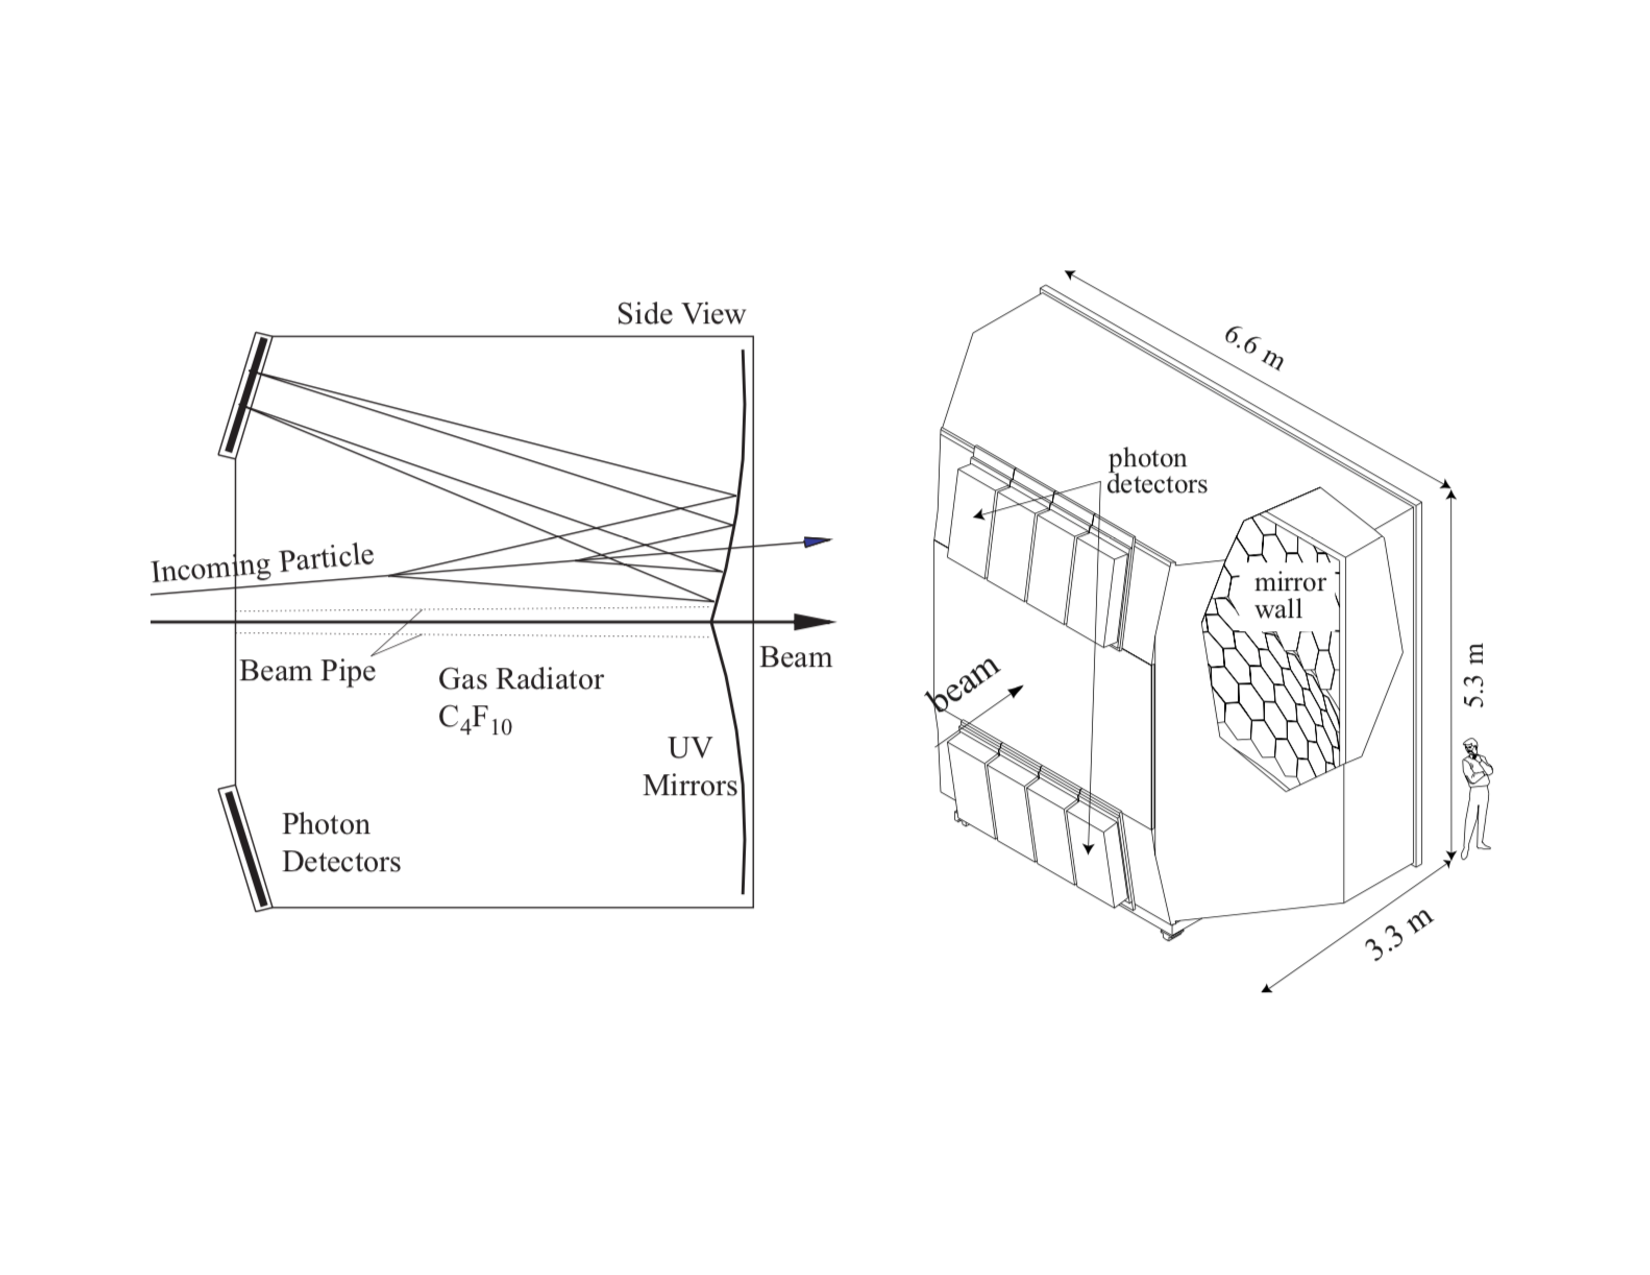
\includegraphics[width=0.6\textwidth]{rich}
  \caption{Side view demonstrating the principle of operation of the RICH
    detector.}
  \label{fig::rich}
\end{figure}

The ECALs and HCALs both stop specific particles of interest where the energy
deposited in each respective calorimeter is proportional to the incoming
particle's energy.  This energy knowledge along the momentum determined from the
tracking detectors allows to determine particle identification.  The ECALs and
HCALs can therefore measure the energy of incoming particles.  The ECALs are
made of lead glass towers with photon multipliers attached to these towers on
one side.  An incoming photon or electron interacts with the lead glass to
produce a light signal which is readout with these photon multipliers.  Other
particles also interact with the material in the ECALs however hadrons and muons
are able to exit through the detector unlike photons and electrons.  A frontal
view of ECAL1 is shown in Fig.~\ref{fig::ECAL1} and a frontal view of ECAL2 is
shown in figure Fig.~\ref{fig::ECAL2}. \par

\begin{figure}[h!t]
  \centering
  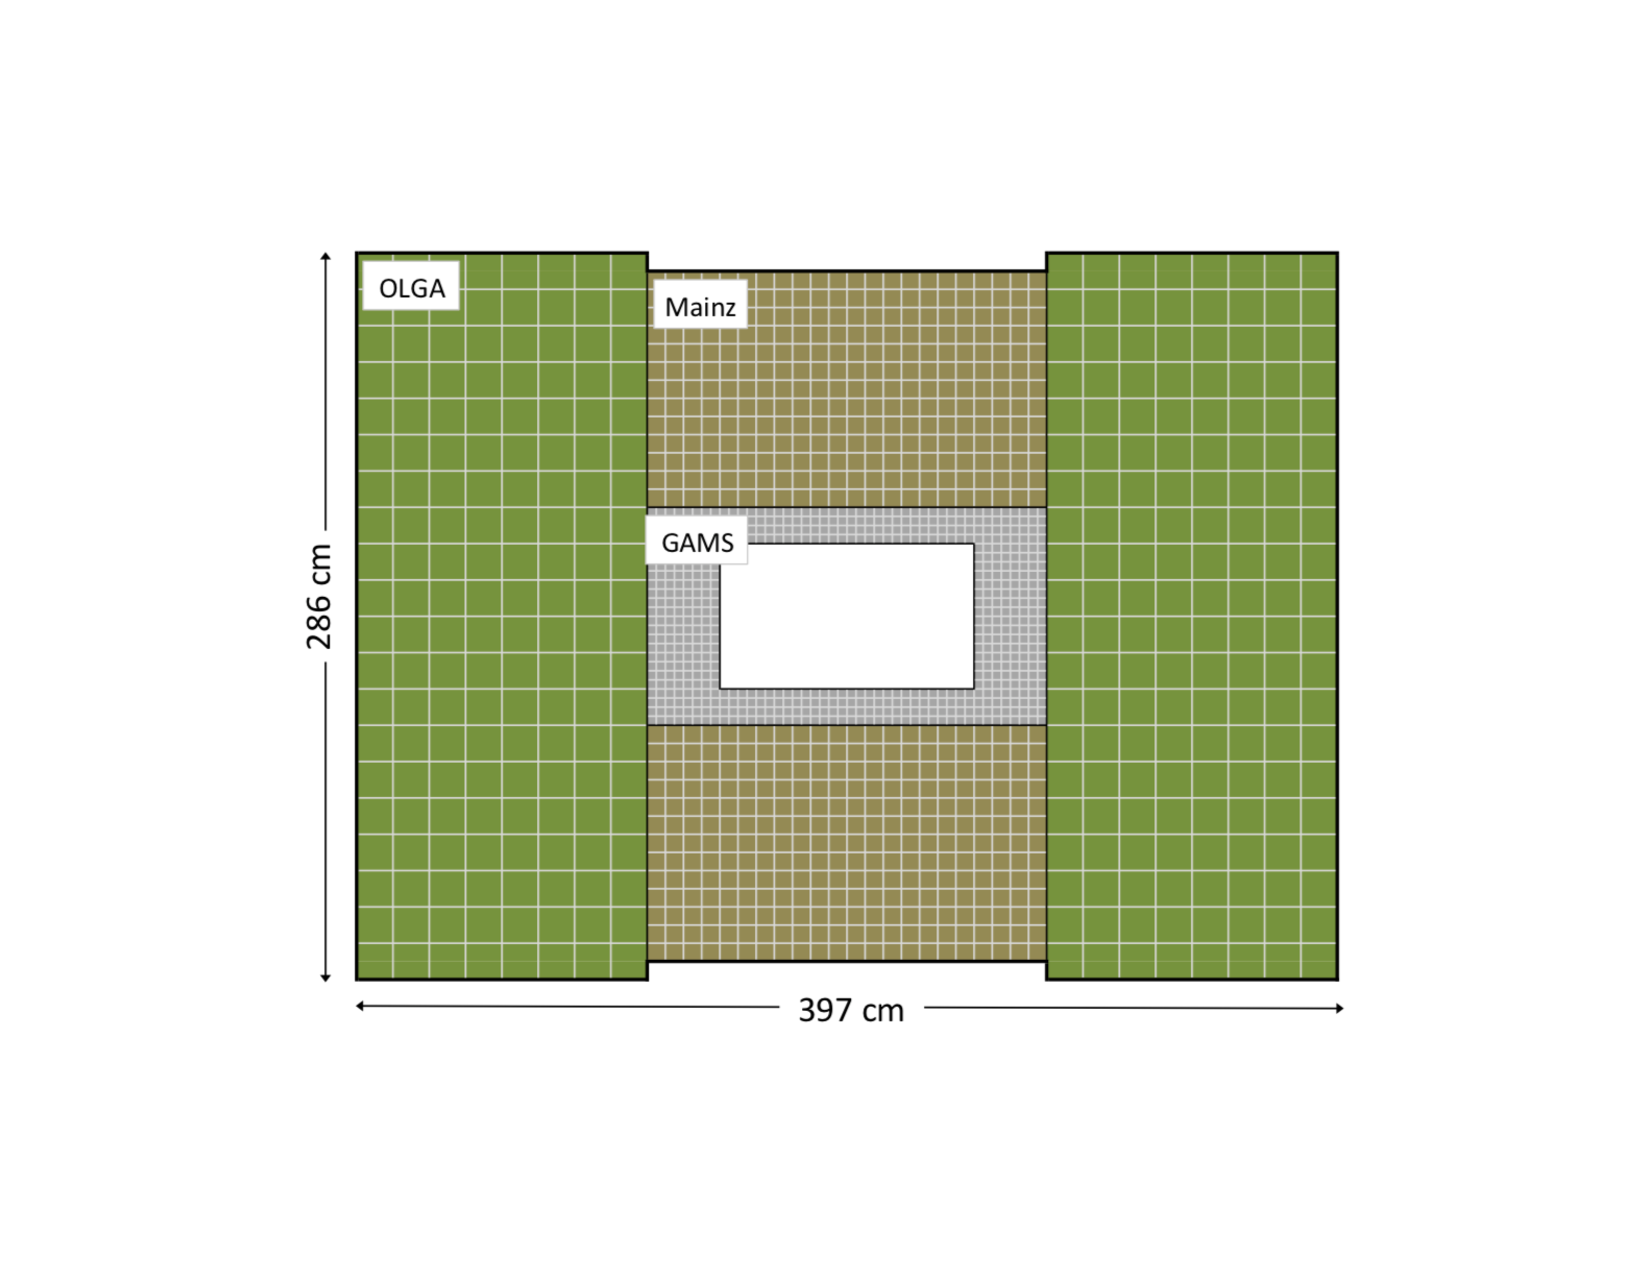
\includegraphics[width=0.6\textwidth]{ECAL1}
  \caption{Frontal view of the electromagnetic calorimeter 1}
  \label{fig::ECAL1}
\end{figure}

\begin{figure}[h!t]
  \centering
  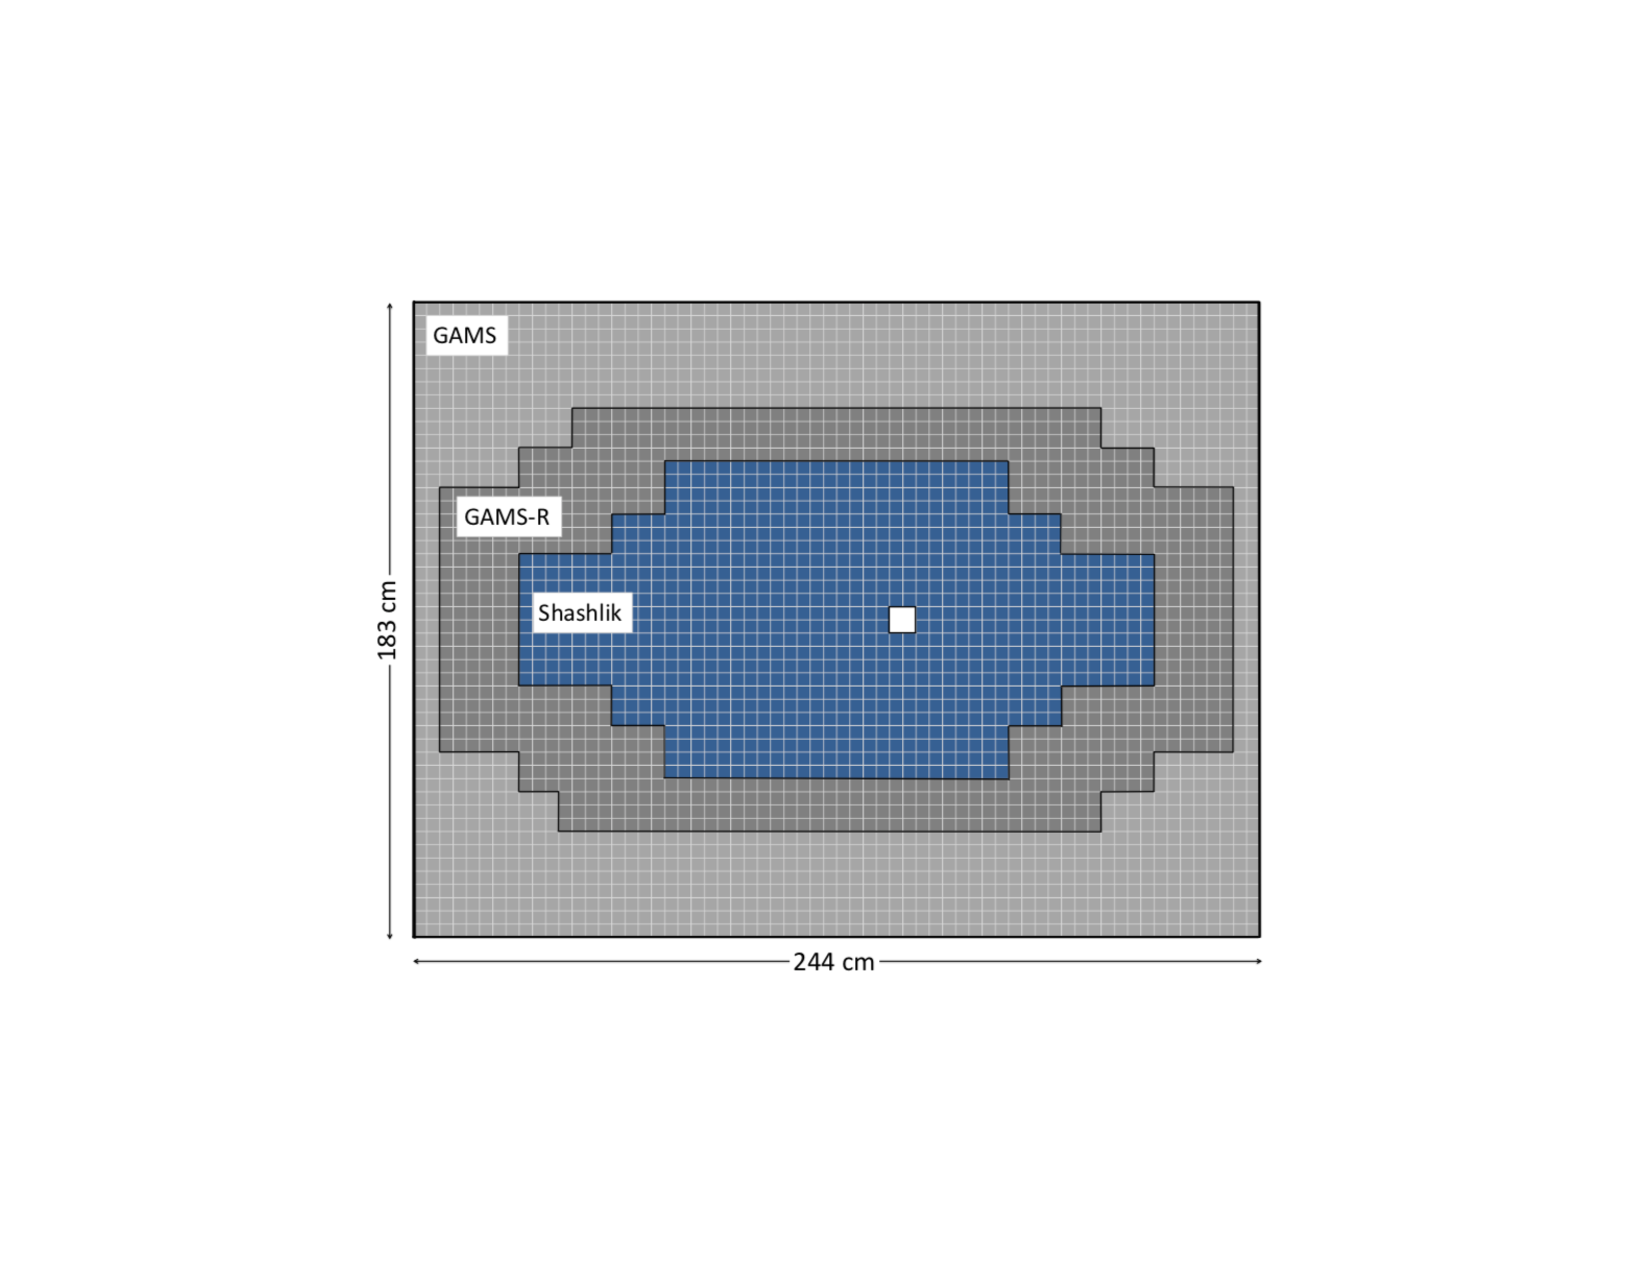
\includegraphics[width=0.6\textwidth]{ECAL2}
  \caption{Frontal view of the electromagnetic calorimeter 2}
  \label{fig::ECAL2}
\end{figure}


The HCALs are sampling calorimeters which are made of alternating layers of iron
and scintillating material.  An incoming hadron deposits all its energy in the
HCAL by making a particle showers in the iron which are detected by photo
multipliers connected to the scintillating material.  The HCALs are placed after
the ECALs in each stage of the spectrometer because an electromagnetic shower
happens faster than a hadronic shower.  The HCALs are affect at determining
particles energy from particle with energies between 10~GeV and 100~GeV. \par

The two MWs are located after an HCAL in their respective stages.  Due to their
higher mass and absence of color charge, muons are able to pass through the most
material budget of any of the particles detected at COMPASS.  For this reason
both MWs consist of an absorber and tracking detectors downstream of this
absorber.  Any particles that make it through the absorber are with a very high
probability muons.  MW1 consists of eight tracking planes before a 60~cm iron
absorber and same number of tracking planes after this absorber.  The tracking
portions of MW1 are build similarly to the richwall, described in
section~\ref{sec::SAT}, in that they are also made of MDT modules.  The active
area of MW1 is 480x410~cm$^2$ and includes a dead zone of 140x80~cm$^2$.  Each
plan of this detector has a spacial resolution of 3~mm.  A sketch of MW1 is
shown in Fig.~\ref{fig::MW1}.  The second muon wall, MW2, is located downstream
of a concrete absorber which 2.4~m thick.  MW2 consists of 12 planes with and
active area of 450x450~cm$^2$ and a dead zone of 90x70~cm$^2$.  The detector
operates similarly to the straw detectors, section~\ref{sec::SAT}, in that it is
made of drift tubes with a wire in the center of these tubes.  The diameter
these drift tubes is 29~mm and the position resolution is about 1.4~mm. \par

\begin{figure}[h!t]
  \centering
  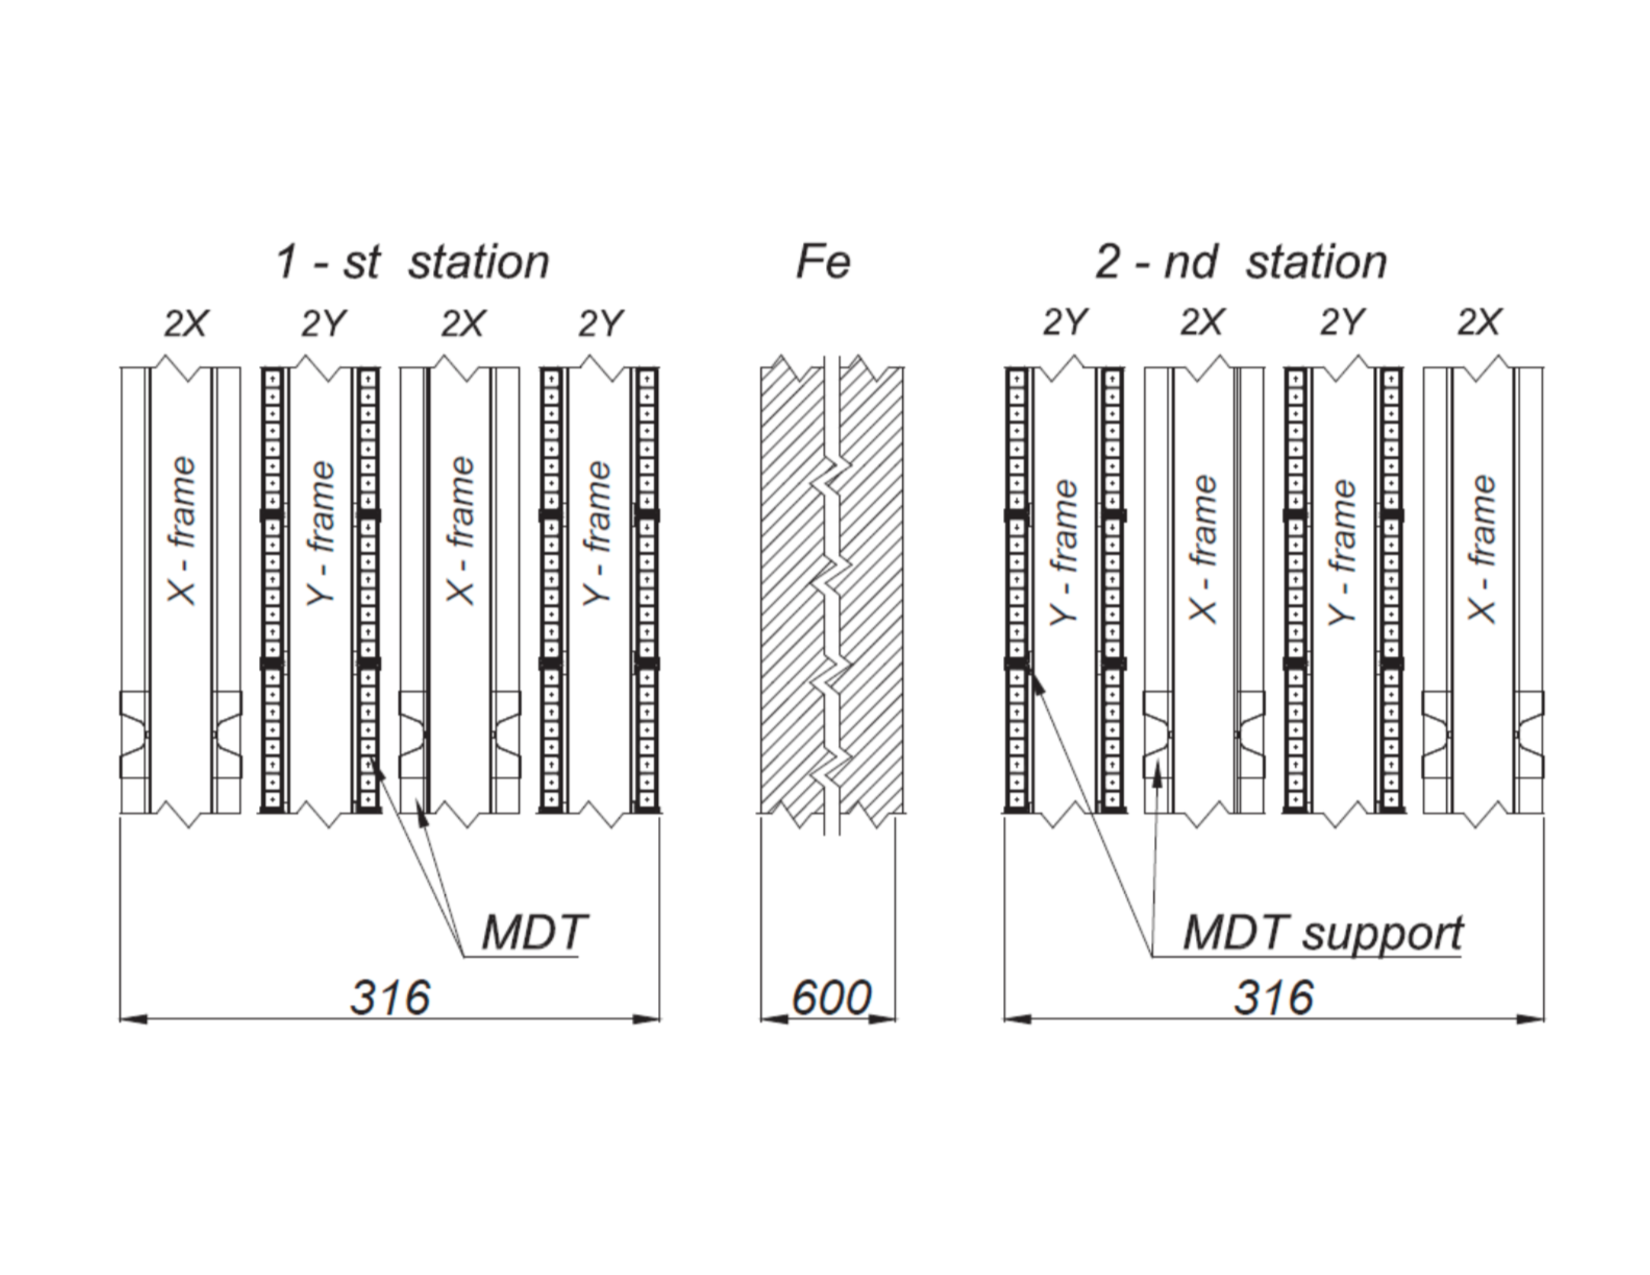
\includegraphics[width=0.7\textwidth]{MW1}
  \caption{A side view sketch of the muon wall 1 detector}
  \label{fig::MW1}
\end{figure}

There is one last absorber in the COMPASS spectrometer located before the H5
hodoscope at the end of the spectrometer hall.  This absorber is called muon
filter 3 (MW3) and ensures that the inner trigger is only triggered by a
muon. \par


\section{Trigger}

\section{Data Acquisition}

\section{Data Production}

\section{2015 Drell-Yan Setup}


This section of the spectrometer covers high
$Q^2$ and high $x_b$.  The target-pointing trigger system in LAS consists of two
hodoscopes, one down stream of the last tracker in LAS and the other just after
an iron muon filter in front of the second spectrometer magnet.

The trigger in SAS is
similar to the LAS trigger but for muons of a lower $Q^2$ value.  The tracking
detectors used in both spectrometers are gaseous detectors (drift chambers,
straws, multi-wire proportional detectors), micro-megas, and gas electron
multiplier (GEM) detectors.  The two stages are separated by two spectrometer
magnets: SM1, with a magnetic field integral of 1~Tm and SM2, with a magnetic
field integral of 4.4~Tm~\cite{compassSpec}.

Both SM1 and SM2 have magnetic
fields in the vertical direction meaning charged particles are deflected in the
x-z plane and can therefore have their momentum determined.  For beam
reconstruction there is a beam telescope upstream of the target consisting of
eight planes of scifi detectors.  To account for the transverse magnetic field
in the polarized target a chicane magnet system was added in the beam line.
This meant that the beam entered at a slight angle in the beam telescope but
exited the target going straight. \par

In 2015, COMPASS took nine data periods labeled W07-W15.  Each data period
lasted two weeks and the spin orientation of the targets was reversed after the
first week of every period to reduce systematic effects arising from different
geometric acceptances and luminosities of up and downstream target cells.
%Most notably the spin
%orientation was reversed to have equal luminosity and to force equal
%geometrical acceptance between the two spin states. \par

For the 2015 Drell-Yan data taking a hadron absorber,
see figure~\ref{fig::Absorber}, was placed just downstream of the target
cells.  This was done to reduce the amount of hadrons and electrons
detected in the spectrometer and therefore ensured a cleaner di-muon
sample.  The absorber material was mostly alumina (Al$_2$O$_3$) and
concrete and the absorber corresponded to approximately 7.5
interactions lengths of material.  Inside the absorber was an aluminum
target followed by a tungsten plug, each of radius 2.5 cm, which acted
as a beam dump.  The aluminum target and tungsten plug served the
double purposes as absorbers and also as unpolarized nuclear targets.
In addition a thin $^6\mathrm{Li}$ absorber was added just downstream of the
primary absorber to absorb thermal neutrons produced in the primary
absorber.  This $^6\mathrm{Li}$ absorber was proposed to improve the
performance of the first tracking detector downstream of the
target. \par

\subsection{DAQ and Reconstruction}
The data acquisition system (DAQ) was recording events at a rate of
approximately 30~kHz with a dead time of 10\%.  In 2015, COMPASS
recorded approximately 750~terabytes of raw data from the nine,
two-week periods.  Raw data refers solely to individual detector
timing and wire or strip positions and does not correspond to physics
observables of interest.  From this raw information the CORAL
reconstruction software at COMPASS is able to determine the trajectory
and momentum of charged particles going through the COMPASS
spectrometer.

%This reconstruction stage reduces the data volume by approximately a factor of 10.
